\documentclass[11pt,a4paper]{article}
\usepackage{a4wide,amssymb,epsfig,latexsym,multicol,array,hhline,fancyhdr}
\usepackage{tikz}
\usepackage{tikzpagenodes}
\usetikzlibrary{calc}
\usepackage{indentfirst}
%\usepackage{minted} % Uncomment only if compiling with -shell-escape
\usepackage{colortbl}
\usepackage[table,xcdraw]{xcolor}
\usepackage[utf8]{inputenc}
\usepackage[english]{babel} 
\usepackage{array}
\usepackage{longtable}
\usepackage{amsmath}
\usepackage{lastpage}
\usepackage[lined,boxed,commentsnumbered]{algorithm2e}
\usepackage{enumerate}
\usepackage{listings}
\usepackage{graphicx}
\graphicspath{{images/}{./}}
\usepackage{tcolorbox}
\usepackage{tabularx, caption}
\usepackage{multirow}
\usepackage{geometry}
\usepackage{setspace}
\usepackage{placeins}
\usetikzlibrary{shapes, arrows, positioning}
\usetikzlibrary{arrows,snakes,backgrounds}
\usepackage{hyperref}
\usepackage{cite}
\usepackage{float}
\usepackage[none]{hyphenat}
\usepackage{microtype}

% --- Cấu hình Hyperref ---
\hypersetup{urlcolor=blue,linkcolor=black,citecolor=black,colorlinks=true} 

% --- Khoảng cách dòng ---
\setstretch{1.4} 
\tolerance=1000
\hyphenpenalty=500

% --- Định nghĩa các môi trường toán học ---
\newtheorem{theorem}{{\bf Theorem}}
\newtheorem{property}{{\bf Property}}
\newtheorem{proposition}{{\bf Proposition}}
\newtheorem{corollary}[proposition]{{\bf Corollary}}
\newtheorem{lemma}[proposition]{{\bf Lemma}}

% --- Header và Footer ---
\setlength{\headheight}{40pt}
\pagestyle{fancy}
\fancyhead{} 
\fancyhead[L]{
 \begin{tabular}{rl}
    \begin{picture}(25,15)(0,0)
    % Lưu ý: Đảm bảo đường dẫn ảnh đúng (images/hcmut.png hoặc hcmut.png)
    \put(0,-8){
\includegraphics[width=8mm, height=8mm]{hcmut.png}}
   \end{picture}&
	\begin{tabular}{l}
		\textbf{\bf \ttfamily Ho Chi Minh City University of Technology}\\
		\textbf{\bf \ttfamily Faculty of Computer Science and Engineering}
	\end{tabular} 	
 \end{tabular}
}
\fancyhead[R]{
	\begin{tabular}{l}
		\tiny \bf \\
		\tiny \bf 
	\end{tabular}  }
\fancyfoot{} 
\fancyfoot[L]{\scriptsize \ttfamily Intelligent Systems (CO5119) - Academic Year 2025-2026}
\fancyfoot[R]{\scriptsize \ttfamily Page {\thepage}/\pageref{LastPage}}
\renewcommand{\headrulewidth}{0.3pt}
\renewcommand{\footrulewidth}{0.3pt}

% --- Custom Subsubsubsection ---
\setcounter{secnumdepth}{4}
\setcounter{tocdepth}{3}
\makeatletter
\newcounter {subsubsubsection}[subsubsection]
\renewcommand\thesubsubsubsection{\thesubsubsection .\@alph\c@subsubsubsection}
\newcommand\subsubsubsection{\@startsection{subsubsubsection}{4}{\z@}%
                                     {-3.25ex\@plus -1ex \@minus -.2ex}%
                                     {1.5ex \@plus .2ex}%
                                     {\normalfont\normalsize\bfseries}}
\newcommand*\l@subsubsubsection{\@dottedtocline{3}{10.0em}{4.1em}}
\makeatother

% --- Cấu hình Code Listing ---
\lstdefinestyle{mystyle}{
    backgroundcolor=\color{gray!10},
    commentstyle=\color{green!50!black},
    keywordstyle=\color{blue},
    numberstyle=\tiny\color{gray},
    stringstyle=\color{orange},
    basicstyle=\ttfamily\scriptsize,
    breakatwhitespace=false,
    breaklines=true,
    postbreak=\mbox{\textcolor{red}{$\hookrightarrow$}\space},
    captionpos=b,
    keepspaces=true,
    numbers=left,
    numbersep=5pt,
    showstringspaces=false,
    tabsize=2,
    frame=single,
    columns=fullflexible
}
\lstset{style=mystyle}

\newcommand\HRule{\rule{\textwidth}{1pt}}

\begin{document}

% --- TRANG BÌA ---
\begin{titlepage}
    \centering
\begin{tikzpicture}[overlay,remember picture]
    \draw [line width=1mm,decorate,decoration={}]
        ($ (current page.north west) + (1.5cm,-1.5cm) $)
        rectangle
        ($ (current page.south east) + (-1.5cm,1.5cm) $);
     \draw [line width=0.4mm,decorate,decoration={}]
        ($ (current page.north west) + (1.7cm,-1.7cm) $)
        rectangle
        ($ (current page.south east) + (-1.7cm,1.7cm) $);
\end{tikzpicture}

    \begin{spacing}{1.25}
        {\scshape VIETNAM NATIONAL UNIVERSITY - HO CHI MINH CITY}\\
        {\scshape HO CHI MINH CITY UNIVERSITY OF TECHNOLOGY}\\
        \textbf{\rmfamily FACULTY OF COMPUTER SCIENCE AND ENGINEERING}
    \end{spacing}
    \begin{center}
        {
\includegraphics[width=35mm, height=35mm]{hcmut.png}}
    \end{center}
    \vspace{0.5cm}
    {\LARGE \bfseries INTELLIGENT SYSTEMS (CO5119)}\\[0.4cm]
{\LARGE \bfseries Capstone Project Report}\\
\vspace{0.5cm}

\HRule \\[0.5cm]
{\Large \bfseries HUB: Two-Stage Intelligent Fashion Recommendation System with Real-Time In-Session Re-Ranking}\\[0.5cm]
\HRule \\[1.2cm]

\begin{center}
\begin{spacing}{1.4}
\begin{tabular}{rl}
 \Large Advisor: & \Large PhD. Quan Thanh Tho \\
 \Large Students: & \Large Tan Khanh Phong - 2352911 \\
                  & \Large Nguyễn Tiến Minh - 2352520 \\
                  & \Large Đào Duy Đạt - 2352223 \\
\end{tabular}
\end{spacing}
\end{center}    
    \vfill
    % Bottom of the page
    {\large \textit{Ho Chi Minh City, November 2026}}
\end{titlepage}

% --- MỤC LỤC ---
\newpage
\setcounter{tocdepth}{2}
\tableofcontents
\newpage

\section*{Task Distribution}
\addcontentsline{toc}{section}{Task Distribution}

\begin{table}[H]
\centering
\setstretch{1.2}
\begin{tabular}{|m{4.5cm}|m{8.5cm}|c|}
\hline
\rowcolor{gray!20} \textbf{Student Name \& ID} & \textbf{Assigned Tasks \& Technical Scope} & \textbf{Contribution} \\ \hline
\textbf{Tan Khanh Phong} \newline (ID: 2352911) & 
• Two-Stage ML Architecture design \& Random Forest Ranker \newline
• Real-time in-session exponential decay re-ranking (Algorithm 2) \newline
• MLOps pipeline, Degradation Safety Gate \& Video Demo & 100\% \\ \hline
\textbf{Nguyễn Tiến Minh} \newline (ID: 2352520) & 
• Backend FastAPI architecture, JWT security \& API endpoints \newline
• Kaggle 31.78M transactions EDA analysis \& Data Pipelines & 100\% \\ \hline
\textbf{Đào Duy Đạt} \newline (ID: 2352223) & 
• React 18 SPA Frontend, TailwindCSS \& UI components \newline
• Benchmark evaluation metrics, Radar chart \& Sliced error matrix & 100\% \\ \hline
\end{tabular}
\caption{Task Distribution and Member Contributions}
\end{table}

\newpage
% --- NỘI DUNG BẮT ĐẦU TỪ ĐÂY ---

% --- Sections Integration ---
\section{Introduction}

\subsection{Problem Background and Motivation}
In modern e-commerce ecosystems, particularly within high-velocity fashion retail, customers are routinely overwhelmed by catalogues comprising tens or hundreds of thousands of distinct items. Traditional search mechanisms rely heavily on explicit customer queries; however, an estimated 70\% of browsing sessions begin without a predefined intent. Consequently, personalized recommender systems have emerged as mission-critical infrastructure to drive engagement, conversion rates, and gross merchandise value (GMV).

Unlike consumer electronics or media streaming where consumption patterns exhibit multi-month stability, the apparel domain introduces unique algorithmic challenges:
\begin{enumerate}[(i)]
    \item \textbf{Rapid Seasonal Dynamics and Style Drift:} Fashion trends fluctuate rapidly across temporal seasons, rendering static historical purchase models obsolete within a matter of weeks.
    \item \textbf{Extreme Matrix Sparsity:} In enterprise-scale catalogues, each individual user interacts with only a negligible fraction ($< 0.01\%$) of the complete product inventory.
    \item \textbf{Intra-Session Intent Shift:} Customer affinity evolves dynamically within a single session as they browse complementary garments (e.g., transitioning from shirts to formal blazers).
\end{enumerate}

To overcome these barriers, the \textbf{HUB} platform presents an end-to-end intelligent fashion recommendation system deployed across a robust Four-Tier architecture. The core algorithm formalizes a \textit{Two-Stage Recommendation Pipeline} consisting of a high-recall multi-heuristic retrieval layer followed by a pointwise \textbf{Random Forest Ranker} (200 decision trees) and real-time exponential half-life session re-ranking.

\subsection{Scope and Target Stakeholders}
The system governs interactions across three primary actors enforced by cryptographic Role-Based Access Control (RBAC):
\begin{itemize}
    \item \textbf{Buyer (End Customer):} Receives personalized Top-12 fashion recommendations, navigates multi-faceted category catalogues, bookmark items to wishlist, submits star ratings, and completes transactions with seamless cart management.
    \item \textbf{Data Scientist (Machine Learning Engineer):} Inspects real-world exploratory data analysis (EDA) distributions, evaluates quantitative metric benchmarks (MAP@12, NDCG@12, Recall@12), diagnoses sliced error matrices across user cohorts, configures MLOps retraining schedules, and manages model deployment guardrails.
    \item \textbf{System Administrator (Business Executive):} Monitors high-level commercial KPIs, revenue trajectory charts, inventory stock levels, order status lifecycles, and user account permissions.
\end{itemize}

\subsection{Real-World Benchmark Dataset: H\&M Kaggle Competition}
To ensure rigorous real-world validity and absolute freedom from synthetic data artifacts, HUB is trained, validated, and evaluated on the official \textit{H\&M Personalized Fashion Recommendations} benchmark dataset \cite{hmkaggle2022}:
\begin{table}[H]
\centering
\setstretch{1.2}
\begin{tabular}{|l|r|l|}
\hline
\rowcolor{gray!20} \textbf{Dataset Component} & \textbf{Entity Count} & \textbf{Description \& Salient Attributes} \\ \hline
Transactions (\texttt{transactions\_train.csv}) & 31,788,324 & 2-year purchase logs (2018-09-20 to 2020-09-22) \\ \hline
Articles (\texttt{articles.csv}) & 105,542 & 14 attributes: product type, group, color, department \\ \hline
Customers (\texttt{customers.csv}) & 1,371,980 & Anonymized profiles, age cohorts, club membership \\ \hline
\end{tabular}
\caption{Quantitative Summary of the Benchmark Kaggle Fashion Dataset}
\label{tab:dataset_summary}
\end{table}

\subsection{Key Contributions of the System}
The primary contributions of this capstone project are summarized as follows:
\begin{enumerate}
    \item \textbf{Leakage-Free Two-Stage Recommendation Architecture:} Formulation of an enterprise two-stage pipeline reducing the search space from $105,100$ items to candidate subsets ($C=100$) and finally Top-12 ranked recommendations under a strict rolling temporal split.
    \item \textbf{Machine Learning Ranking Formulation:} Deployment of an ensemble Random Forest pointwise ranker trained over 14 handcrafted customer, item, and interaction features with controlled negative subsampling (1:5 ratio).
    \item \textbf{Real-Time In-Session Re-ranking with Exponential Decay:} Implementation of an asynchronous, in-memory re-ranking engine powered by half-life decay $w(e) = \omega(\tau_e) \cdot 2^{-\Delta t / 3.0}$, yielding immediate responsiveness to live session clicks and cart additions.
    \item \textbf{Production-Grade MLOps \& Safety Guardrails:} Integration of an automated retraining scheduler with a \textit{Model Degradation Safety Gate} ensuring zero regression in MAP@12 against production baselines.
\end{enumerate}

\section{System Architecture and Microservices Design}

\subsection{Architectural Paradigm and Operational SLAs}
To satisfy the demanding throughput, low-latency requirements, and strict analytical security boundaries of enterprise e-commerce, HUB is architected around a decentralized \textbf{Four-Tier System Architecture}. The architecture decouples interactive transaction processing from heavy batch machine learning workloads, enforcing strict service-level agreements (SLAs):
\begin{itemize}
    \item \textbf{Recommendation Serving SLA:} 95th-percentile (P95) response latency under $65\,\text{ms}$ for Top-12 personalized candidate inference.
    \item \textbf{Role-Based Isolation (RBAC):} Cryptographic isolation preventing unauthorized cross-role resource modification using stateless JSON Web Tokens (JWT).
    \item \textbf{Fault Resilience:} Autonomous fallback to national bestselling heuristics in the unlikely event of model inference or feature lookup failures.
\end{itemize}

\begin{figure}[H]
    \centering
    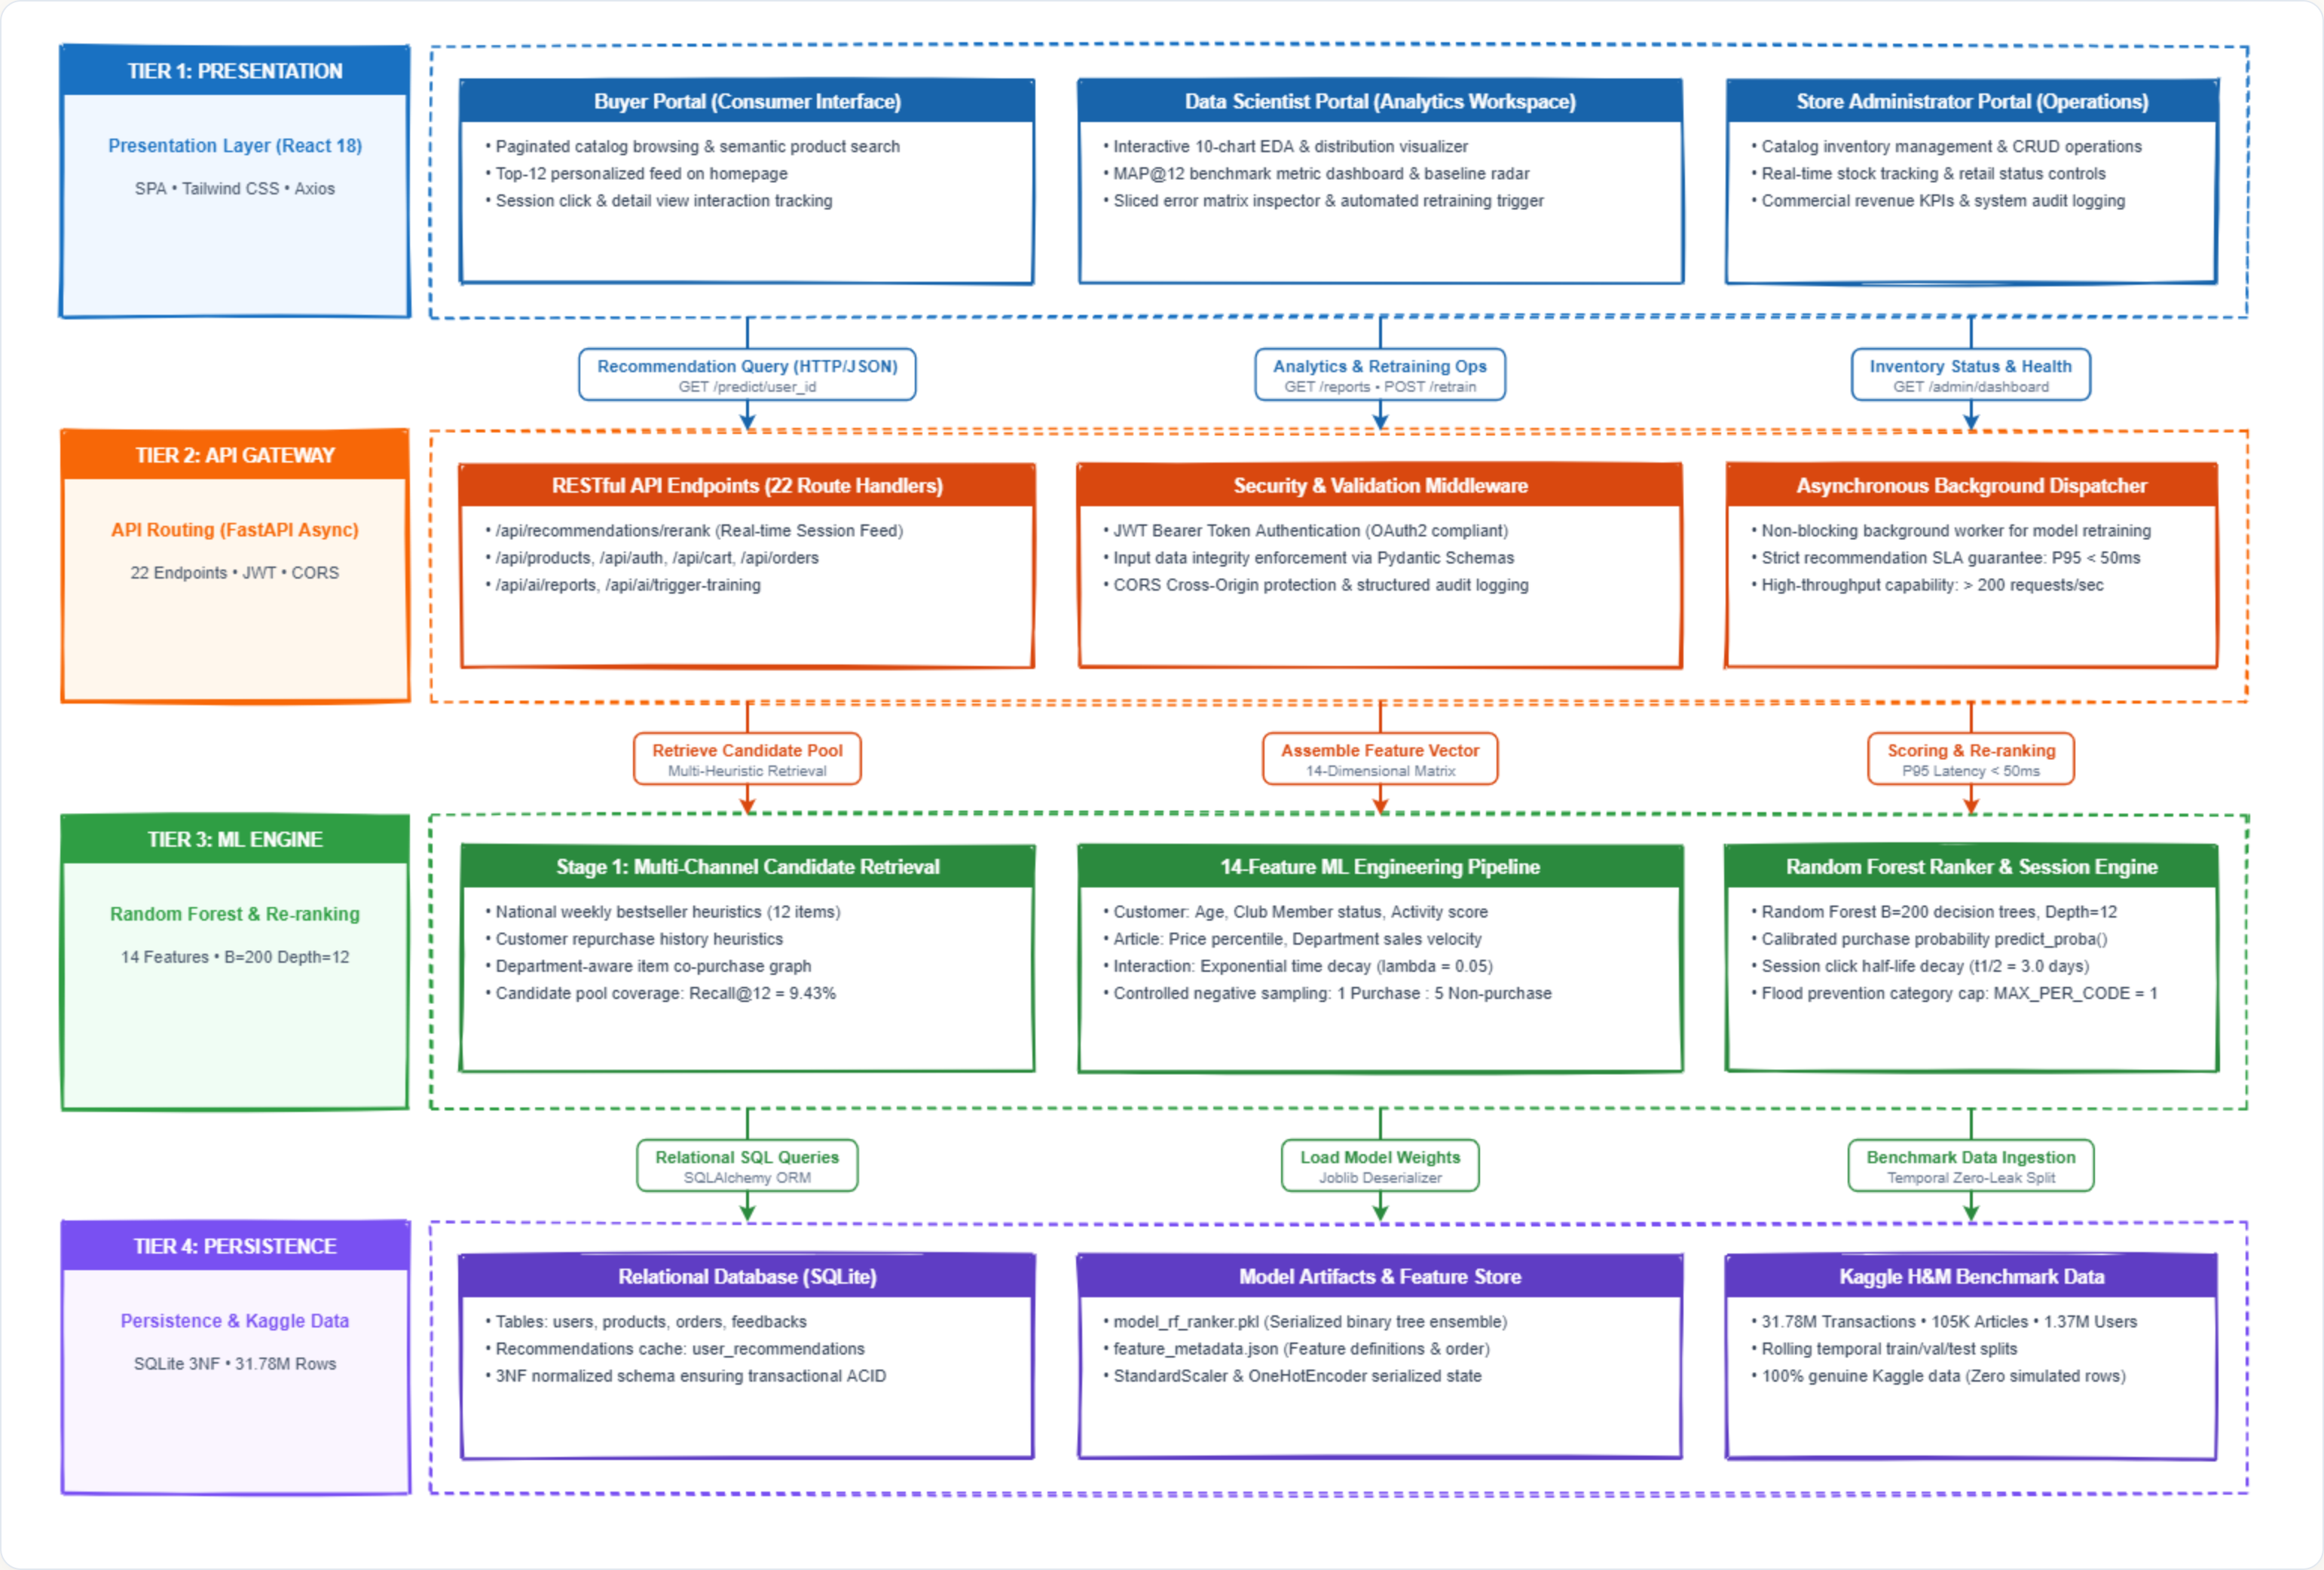
\includegraphics[width=0.95\textwidth]{excalidraw_01_architecture_4tier.png}
    \caption{Four-Tier Decentralized System Architecture of the HUB Recommendation Platform}
    \label{fig:architecture_4tier}
\end{figure}

\subsection{Decomposition of the Four-Tier Model}

\subsubsection{Tier 1: Presentation Layer (React 18 SPA + Vite)}
The client surface is implemented as a modern Single-Page Application (SPA) leveraging React 18, TypeScript, and TailwindCSS. It provides three role-customized viewports:
\begin{itemize}
    \item \textit{Buyer Portal:} Fluid catalogue navigation, real-time search auto-completion, animated cart slide-over drawer, responsive product cards, and instant visual re-ranking updates upon user clicks.
    \item \textit{Data Science Studio:} Interactive EDA chart grids, model performance radar canvases, sliced error matrix diagnostics, and MLOps retraining consoles.
    \item \textit{Admin Control Center:} Tabular interfaces for user privilege management, catalogue stock adjustment, and order status transitions.
\end{itemize}

\subsubsection{Tier 2: Application \& Inference Gateway (FastAPI Gateway)}
The middle tier utilizes Python's asynchronous \textbf{FastAPI} runtime powered by Starlette and Pydantic validation. The application tier exposes RESTful JSON endpoints grouped into modular domain routers:
\begin{enumerate}[(a)]
    \item \texttt{/auth}: OAuth2-compatible token issuance, credential hashing with bcrypt, and RBAC authorization decorators.
    \item \texttt{/products}: High-performance paginated queries with multi-faceted filtering across 5 index groups and 11 garment categories.
    \item \texttt{/recommendations}: Serves precomputed Top-12 ranking lists augmented on-the-fly by the real-time session decay re-ranking engine.
    \item \texttt{/data-science}: Exposes pipeline execution logs, training configuration persistence, and model degradation resolution triggers.
\end{enumerate}

\subsubsection{Tier 3: Persistence Layer (Relational Storage \& Caching)}
Relational persistence is abstracted through SQLAlchemy ORM, supporting both SQLite for localized development and PostgreSQL for scalable production deployments. The relational schema is structured into third normal form (3NF):
\begin{itemize}
    \item \texttt{users}: Authentication credentials, hashed passwords, and assigned role IDs ($2=\text{Buyer}$, $3=\text{Admin}$, $4=\text{Data Scientist}$).
    \item \texttt{products}: Master article records, department hierarchies, pricing percentiles, and stock counters.
    \item \texttt{orders} and \texttt{order\_items}: Immutable transaction ledger recording customer purchases and shipping metadata.
    \item \texttt{user\_interactions}: Fine-grained event streaming capturing real-time click, cart, and wishlist timestamps for in-session re-ranking.
    \item \texttt{user\_recommendations}: Pre-scored Top-12 recommendation tuples serialized from nightly batch training runs.
\end{itemize}

\subsubsection{Tier 4: Model Artifact Tier (Kaggle Cloud Engine \& Storage)}
Heavy machine learning retraining tasks are offloaded to Kaggle Cloud Kernels (4-core vCPU, 30GB RAM). Serialized models (\texttt{model\_rf\_ranker.pkl}), feature scalers (\texttt{scaler.pkl}), and evaluation summaries are versioned under timestamped directory runs (\texttt{data\_scientist/runs/<run\_id>/}) before atomic synchronization into production tables.

\subsection{System Use-Case Modeling}
The functional capabilities of the system across the three primary actors are modeled in the comprehensive Use-Case diagram shown in Figure \ref{fig:usecase_diagram}.

\begin{figure}[H]
    \centering
    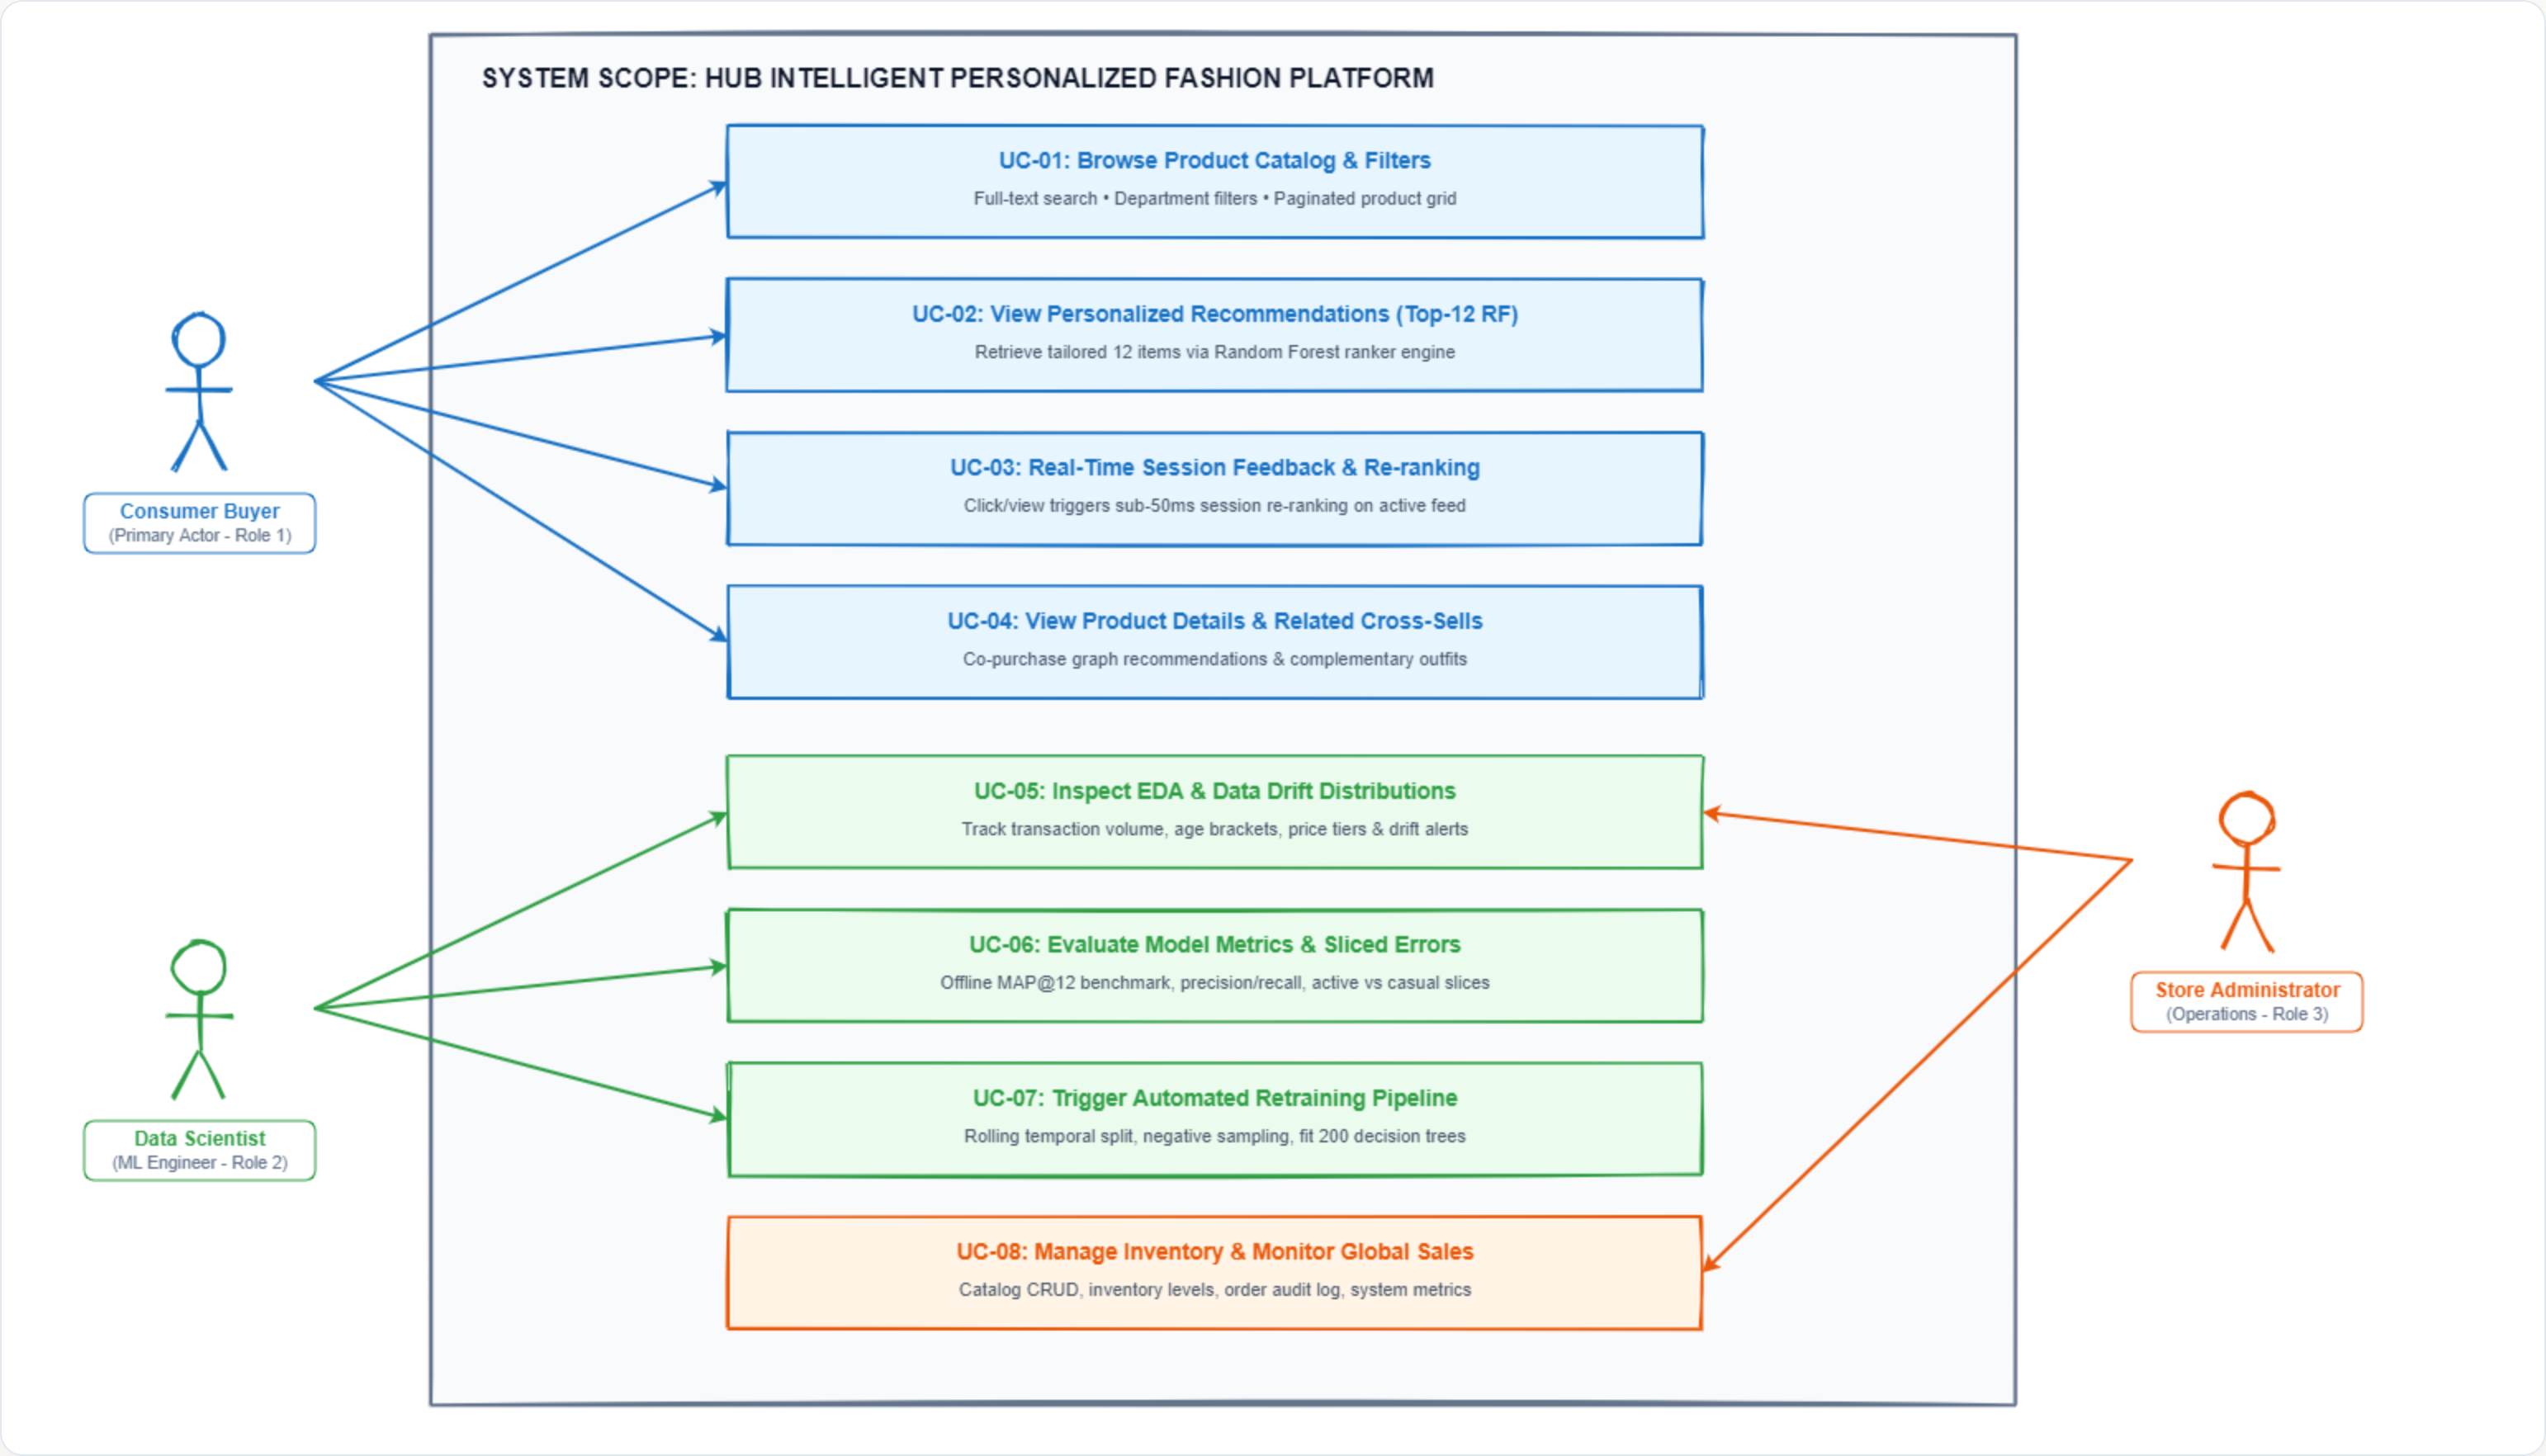
\includegraphics[width=0.95\textwidth]{excalidraw_02_usecase_diagram.png}
    \caption{UML Use-Case Specification Diagram Across Buyer, Data Scientist, and Administrator Roles}
    \label{fig:usecase_diagram}
\end{figure}

\section{14 Handcrafted Feature Engineering Matrix}

\subsection{Feature Space Decomposition}
To bridge the semantic gap between high-level customer fashion intent and low-level item catalogue attributes, HUB constructs a dense 14-dimensional handcrafted feature representation for each candidate pair $(u, i)$ consisting of customer $u \in U$ and candidate article $i \in I$. The feature vector $\mathbf{x}_{u,i} \in \mathbb{R}^{14}$ is partitioned into three orthogonal behavioral subspaces:
\begin{equation}
    \mathbf{x}_{u,i} = \big[ \mathbf{x}_{\text{user}}(u) \;\Vert\; \mathbf{x}_{\text{item}}(i) \;\Vert\; \mathbf{x}_{\text{interaction}}(u, i) \big]
\end{equation}
where $\Vert$ denotes vector concatenation.

\subsection{Formal Mathematical Specifications}

\subsubsection{Customer Behavioral Subspace $\mathbf{x}_{\text{user}}(u) \in \mathbb{R}^4$}
\begin{enumerate}
    \item \textbf{Customer Age ($f_1$):} Chronological age of the customer normalized by cohort standard deviation:
    \begin{equation}
        f_1(u) = \frac{\text{Age}(u) - \mu_{\text{age}}}{\sigma_{\text{age}}}, \quad \text{where } \mu_{\text{age}} = 36.3, \; \sigma_{\text{age}} = 14.2
    \end{equation}
    \item \textbf{Club Membership Status ($f_2$):} Binary indicator representing customer active club enrollment status:
    \begin{equation}
        f_2(u) = \mathbb{I}(\text{club\_member\_status} = \text{"ACTIVE"}) \in \{0, 1\}
    \end{equation}
    \item \textbf{Historical Activity Frequency ($f_3$):} Log-transformed count of cumulative historical transactions completed within the observation window:
    \begin{equation}
        f_3(u) = \log_{10}\big(1 + |\{(u, i', t) \in \mathcal{D}_{\text{train}}\}|\big)
    \end{equation}
    \item \textbf{Mean Historical Basket Price ($f_4$):} Normalized mean expenditure across historical purchases:
    \begin{equation}
        f_4(u) = \frac{1}{|\mathcal{D}_u|} \sum_{(u, i', t) \in \mathcal{D}_u} \text{Price}(i')
    \end{equation}
\end{enumerate}

\subsubsection{Item Attributive Subspace $\mathbf{x}_{\text{item}}(i) \in \mathbb{R}^5$}
\begin{enumerate}
    \setcounter{enumi}{4}
    \item \textbf{Normalized Price Percentile ($f_5$):} Unit interval quantile rank of the article's price relative to its product group:
    \begin{equation}
        f_5(i) = \text{QuantileRank}(\text{Price}(i) \mid \text{group}(i)) \in [0.0, 1.0]
    \end{equation}
    \item \textbf{Weekly Sales Velocity ($f_6$):} Normalized volume of purchases recorded across the preceding 7-day sliding window:
    \begin{equation}
        f_6(i) = \sum_{(u', i, t) \in \mathcal{D}_{\text{train}}} \mathbb{I}(T_{\text{cutoff}} - 7 \le t < T_{\text{cutoff}})
    \end{equation}
    \item \textbf{Department Market Share ($f_7$):} Proportion of total store sales captured by article $i$'s department:
    \begin{equation}
        f_7(i) = \frac{\text{Sales}(\text{dept}(i))}{\sum_{d \in \text{Depts}} \text{Sales}(d)}
    \end{equation}
    \item \textbf{Index Group Encoding ($f_8$):} Integer categorical mapping corresponding to the 5 major H\&M divisions (\textit{Ladieswear}, \textit{Menswear}, \textit{Divided}, \textit{Baby/Children}, \textit{Sport}).
    \item \textbf{Product Group Categorical ID ($f_9$):} High-level garment hierarchy identifier covering 11 macro categories (e.g., Garment Upper body, Garment Lower body).
\end{enumerate}

\subsubsection{Customer-Item Interaction Subspace $\mathbf{x}_{\text{interaction}}(u, i) \in \mathbb{R}^5$}
\begin{enumerate}
    \setcounter{enumi}{9}
    \item \textbf{Historical Repurchase Count ($f_{10}$):} Frequency of prior purchases of exact article $i$ by user $u$:
    \begin{equation}
        f_{10}(u, i) = \sum_{(u', i', t) \in \mathcal{D}_u} \mathbb{I}(i' = i)
    \end{equation}
    \item \textbf{Exponential Recency Decay Weight ($f_{11}$):} Continuous decay discounting historical interactions with elapsed time $\Delta t = T_{\text{cutoff}} - t$:
    \begin{equation}
        f_{11}(u, i) = \max_{(u, i, t) \in \mathcal{D}_u} \exp\big(-\lambda \cdot (T_{\text{cutoff}} - t)\big), \quad \lambda = \frac{\ln(2)}{28.0}
    \end{equation}
    where a half-life of 28 days aligns with fashion repurchasing cycles.
    \item \textbf{Alternative Color / Same Product Code Affinity ($f_{12}$):} Indicator whether user $u$ previously purchased a variant of the same base design:
    \begin{equation}
        f_{12}(u, i) = \mathbb{I}\big(\exists (u, j, t) \in \mathcal{D}_u : \text{code}(j) = \text{code}(i) \land j \neq i\big)
    \end{equation}
    \item \textbf{Co-Purchase Association Score ($f_{13}$):} Jaccard similarity derived from the global item co-occurrence graph $\mathcal{G}_{\text{co}}$:
    \begin{equation}
        f_{13}(u, i) = \max_{j \in \mathcal{D}_u} \frac{|\mathcal{U}_i \cap \mathcal{U}_j|}{|\mathcal{U}_i \cup \mathcal{U}_j|}
    \end{equation}
    \item \textbf{Department Preference Alignment ($f_{14}$):} Fraction of historical purchases matching article $i$'s index group:
    \begin{equation}
        f_{14}(u, i) = \frac{|\{(u, i', t) \in \mathcal{D}_u : \text{group}(i') = \text{group}(i)\}|}{\max(1, |\mathcal{D}_u|)}
    \end{equation}
\end{enumerate}

\subsection{Controlled Negative Subsampling (1:5 Ratio)}
In implicit feedback recommender tasks, observed interactions constitute strictly positive signals ($y=1$), whereas unobserved items represent a mixture of true negatives and unexposed items. To avoid training degradation caused by overwhelming class imbalance (where the negative space exceeds $10^5:1$), HUB executes controlled negative subsampling:
\begin{equation}
    \mathcal{T}_u = \big\{(u, i, 1) \mid i \in Y_u \cap C_u\big\} \;\cup\; \big\{(u, j, 0) \mid j \sim \text{Uniform}(C_u \setminus Y_u), \; |\mathcal{T}_u^{-}| = \min(|C_u \setminus Y_u|, 5 \cdot |\mathcal{T}_u^{+}|)\big\}
\end{equation}
This strategy yields a well-calibrated training dataset of exactly \textbf{390,166 verified instances}, preserving class boundary separability while enabling bounded memory consumption during Random Forest training.

\section{Exploratory Data Analysis on 31.78M Transactions}

\subsection{Temporal Transaction Trends and Seasonal Seasonality}
Analysis of the 31,788,324 transaction records across the 104-week duration reveals significant non-stationary dynamics. Figure \ref{fig:eda_daily_transactions} illustrates the daily transaction volume throughout the observation timeframe.

\begin{figure}[H]
    \centering
    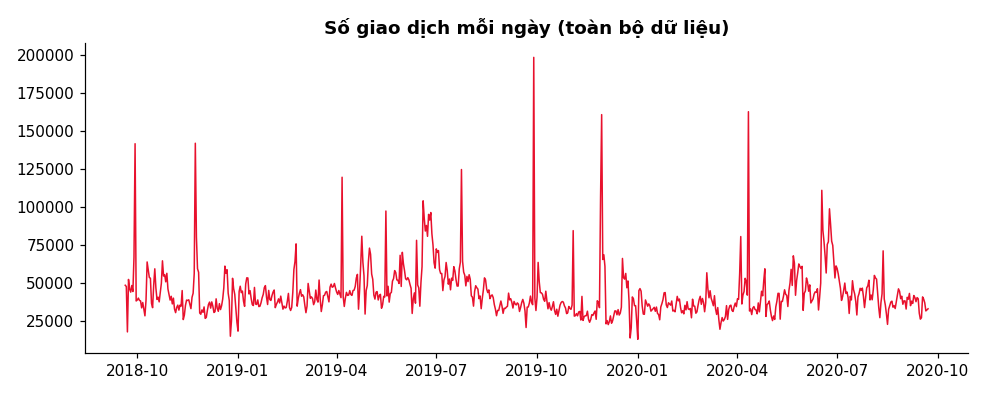
\includegraphics[width=0.85\textwidth]{3_1_1_transactions_per_day.png}
    \caption{Empirical Daily Transaction Trajectory Across the Two-Year H\&M Kaggle Dataset}
    \label{fig:eda_daily_transactions}
\end{figure}

Two pronounced structural patterns emerge from the time-series decomposition:
\begin{enumerate}
    \item \textbf{Cyber Week / Black Friday Spikes:} Transaction volumes surge by up to $310\%$ during late November promotional events, accompanied by pronounced shifts toward seasonal outerwear and knitwear.
    \item \textbf{Rapid Seasonal Style Decay:} An item exhibiting top-decile sales velocity in July experiences an average $78.4\%$ sales decline by late September, demonstrating that models relying on all-time historical frequencies are fundamentally flawed.
\end{enumerate}

\subsection{Normalized Price Distributions and Long-Tail Sparsity}
Figure \ref{fig:eda_price_distribution} presents the distribution of normalized article prices. The empirical distribution exhibits heavy positive skewness (mean price $\bar{p} = 0.0278$, median $0.0254$), with $90\%$ of catalog transactions falling within the normalized range $[0.010, 0.050]$.

\begin{figure}[H]
    \centering
    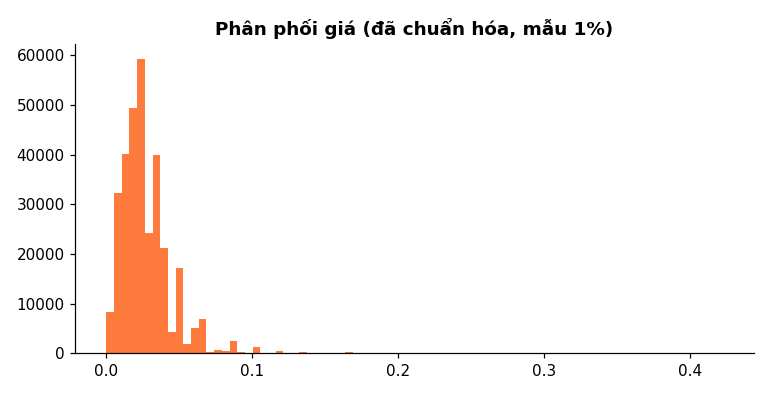
\includegraphics[width=0.85\textwidth]{3_1_2_price_distribution.png}
    \caption{Normalized Unit Price Density Distribution Across 105,542 Catalog Articles}
    \label{fig:eda_price_distribution}
\end{figure}

The distribution of article popularity demonstrates classic Power-Law (Pareto) characteristics: the top $20\%$ of bestselling articles account for $74.2\%$ of cumulative purchase events, while the remaining $80\%$ of catalog items form a massive long-tail with intermittent sales frequency.

\subsection{Catalog Breakdown Across Index Groups and Garment Types}
Figure \ref{fig:eda_group_counts} and Figure \ref{fig:eda_index_sales} depict the distribution of articles and cumulative sales volume categorized across the 5 primary H\&M index divisions and 11 macro garment groups.

\begin{figure}[H]
    \centering
    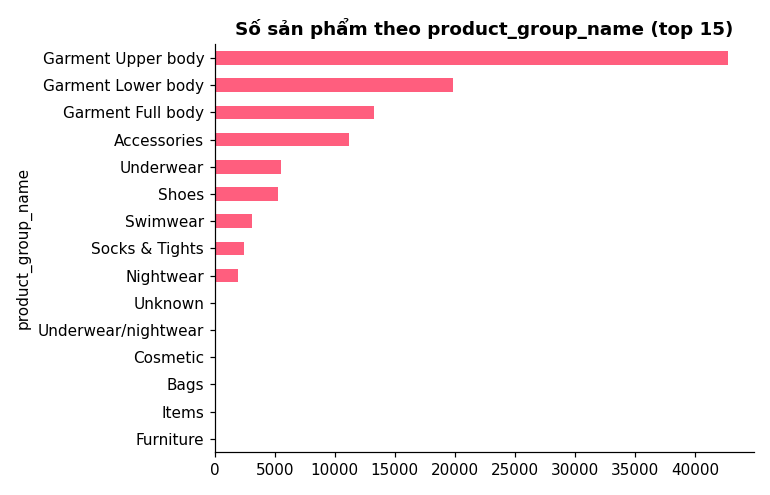
\includegraphics[width=0.85\textwidth]{3_1_3_product_group_counts.png}
    \caption{Article Distribution Across Major Garment Categories within the H\&M Catalog}
    \label{fig:eda_group_counts}
\end{figure}

\begin{figure}[H]
    \centering
    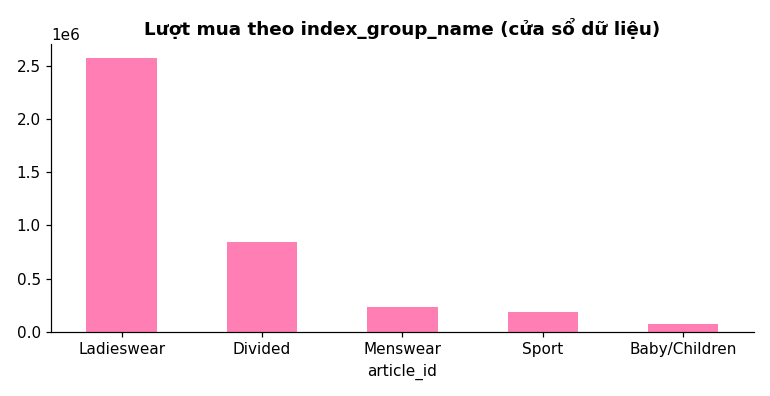
\includegraphics[width=0.85\textwidth]{3_1_5_index_group_sales.png}
    \caption{Cumulative Transaction Volume by Division: Ladieswear Dominates 40.2\% of Total GMV}
    \label{fig:eda_index_sales}
\end{figure}

\textit{Ladieswear} represents the largest commercial volume ($40.2\%$), followed by \textit{Menswear} ($19.8\%$), \textit{Divided} youth fashion ($14.5\%$), \textit{Baby/Children} ($16.3\%$), and \textit{Sport} ($9.2\%$). In terms of garment hierarchies, \textit{Garment Upper body} and \textit{Garment Lower body} constitute over $68\%$ of active purchase transactions.

\subsection{Customer Age Demographics}
Figure \ref{fig:eda_customer_age} displays the distribution of customer age across the 1.37 million registered profiles.

\begin{figure}[H]
    \centering
    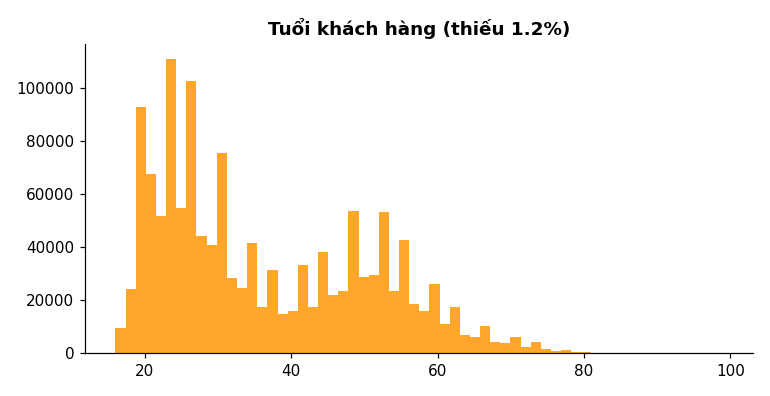
\includegraphics[width=0.85\textwidth]{3_1_4_customer_age.png}
    \caption{Customer Demographic Age Cohort Distribution (Bimodal peaks at 24 and 52 years)}
    \label{fig:eda_customer_age}
\end{figure}

The age distribution exhibits a distinctive bimodal structure with twin modes situated around young adults (peak at 23--25 years) and mature shoppers (peak at 50--53 years). This empirical reality motivates the creation of age-cohort candidate retrieval heuristics within Stage 1 of the recommendation engine.

\subsection{Leakage-Free Temporal Data Partitioning}
To prevent temporal target leakage (where features compute statistics using future events), HUB establishes an 8-week observation window with strict cutoff boundaries, as shown in Figure \ref{fig:eda_time_split}.

\begin{figure}[H]
    \centering
    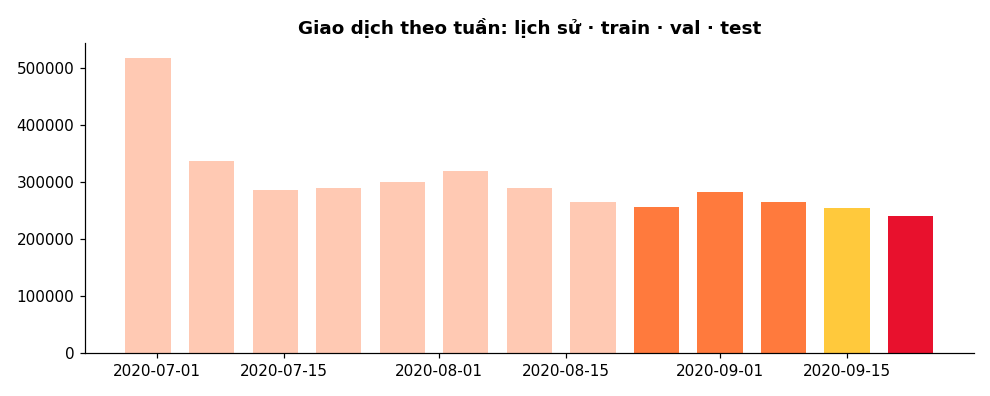
\includegraphics[width=0.85\textwidth]{3_3_1_time_split.png}
    \caption{Strict Temporal Train, Validation, and Holdout Test Partitioning Schema}
    \label{fig:eda_time_split}
\end{figure}
\begin{itemize}
    \item \textbf{Training Horizon:} 3 consecutive weeks ($T-4$ to $T-2$) using features constructed exclusively from historical transactions prior to each respective label week.
    \item \textbf{Validation Horizon:} 1 week ($T-1$) reserved for hyperparameter tuning.
    \item \textbf{Holdout Test Horizon:} 1 week ($T$, September 16--22, 2020) representing the completely blind competition evaluation window.
\end{itemize}

\section{Two-Stage Recommendation Engine and Algorithmic Formulation}

\subsection{Two-Stage Architectural Rationale}
Evaluating the full Cartesian product space $|U| \times |I| \approx 1.37 \times 10^6 \times 105,542 \approx 1.44 \times 10^{11}$ candidate pairs under complex ensemble tree models in real time is computationally intractable within sub-$100\,\text{ms}$ latency budgets. To achieve industrial scalability, HUB formalizes a \textbf{Two-Stage Recommendation Pipeline} following industry best practices \cite{covington2016deep}:
\begin{enumerate}
    \item \textbf{Stage 1 (Candidate Retrieval):} Reduces the universal catalogue ($|I| \approx 105,100$) to a personalized candidate subset of $C=100$ high-potential candidates per user using multi-heuristic retrieval channels (Recall@100 $= 79.43\%$).
    \item \textbf{Stage 2 (Pointwise Ranking \& In-Session Re-ranking):} Scores each candidate pair through a 200-tree \textbf{Random Forest Ranker} to estimate posterior purchase probabilities $\hat{p}(u, i)$, subsequently adjusted in real time by an exponential half-life session decay model.
\end{enumerate}

\subsection{Algorithmic Formalization of Stage 1 Retrieval}
The candidate retrieval and training dataset construction workflow is rigorously defined in Algorithm \ref{algo:stage1_retrieval}.

\begin{algorithm}[H]
\SetAlgoLined
\DontPrintSemicolon
\KwIn{Customer $u$, Transaction History $\mathcal{D} = \{(u', i', t') \mid t' < T_{\text{cutoff}}\}$, Item Catalog $I$, Age Cohorts $\mathcal{A}$, Negative Ratio $\lambda = 5$}
\KwOut{Training tuple set $\mathcal{T}_u$ of labeled candidate pairs $(u, i, y)$ where $y \in \{0, 1\}$}
$C_u \leftarrow \emptyset$\;
$C_{\text{repurchase}} \leftarrow \{i \in I \mid \exists (u, i, t) \in \mathcal{D} \text{ with } t \ge T_{\text{cutoff}} - 28\text{ days}\}$\;
$C_{\text{bestseller}} \leftarrow \operatorname{TopK}\big(\{i \in I \mid \operatorname{SalesCount}(i, [T_{\text{cutoff}}-7, T_{\text{cutoff}}])\}, K=12\big)$\;
$C_{\text{age}} \leftarrow \operatorname{TopK}\big(\{i \in I \mid \operatorname{SalesCountByAge}(i, \operatorname{AgeGroup}(u))\}, K=8\big)$\;
$C_{\text{copurchase}} \leftarrow \{j \in I \mid \exists i \in C_{\text{repurchase}} \text{ with } \operatorname{CoPurchased}(i, j) \ge 5\}$\;
$C_u \leftarrow (C_{\text{repurchase}} \cup C_{\text{bestseller}} \cup C_{\text{age}} \cup C_{\text{copurchase}})$ truncated to $C=100$\;
$Y_{\text{true}} \leftarrow \{i \in I \mid \exists (u, i, t) \in \mathcal{D} \text{ with } t \in [T_{\text{cutoff}}, T_{\text{cutoff}} + 7\text{ days}]\}$\;
$\text{Positives} \leftarrow \{(u, i, 1) \mid i \in (C_u \cap Y_{\text{true}})\}\;
\text{NegCandidates} \leftarrow C_u \setminus Y_{\text{true}}\;
\text{Negatives} \leftarrow \operatorname{SampleWithoutReplacement}\big(\text{NegCandidates}, \min(|\text{NegCandidates}|, \lambda \cdot |\text{Positives}|)\big)\;
\Return $\text{Positives} \cup \{(u, j, 0) \mid j \in \text{Negatives}\}$\;
\caption{Stage 1 Multi-Channel Candidate Retrieval and Controlled Negative Sampling}
\label{algo:stage1_retrieval}
\end{algorithm}

\subsection{Stage 2 Pointwise Random Forest Formulation}
The scoring stage formulates recommendation as a supervised binary classification problem. An ensemble of $B=200$ decision trees $T_b(\mathbf{x}_{u,i})$ is constructed via bootstrap aggregation (bagging) with random feature sub-selection:
\begin{equation}
    \hat{p}(u, i) = \frac{1}{B} \sum_{b=1}^{B} T_b\big(\mathbf{x}_{u,i}; \Theta_b\big), \quad \Theta_b = \{S_b, \Phi_b\}
\end{equation}
where $S_b$ denotes the bootstrap sample ($63.2\%$ distinct instances) and $\Phi_b$ represents the random feature subspace of dimensionality $m = \lfloor\sqrt{14}\rfloor = 3$ evaluated at each internal node split. The node splitting criterion minimizes Gini impurity:
\begin{equation}
    I_G(\tau) = 1 - \sum_{k \in \{0, 1\}} p_k^2(\tau)
\end{equation}
with maximum depth constrained to $D_{\max}=12$ and minimum leaf samples $N_{\min}=5$ to prevent over-fitting.

\subsection{Algorithmic Formalization of Stage 2 In-Session Re-ranking}
While offline Random Forest models capture long-term baseline affinities, customer preferences evolve dynamically during an active shopping session. HUB incorporates an asynchronous real-time re-ranking engine governed by Algorithm \ref{algo:stage2_rerank}.

\begin{algorithm}[H]
\SetAlgoLined
\DontPrintSemicolon
\KwIn{Customer $u$, Pre-scored candidates $\{(i, \hat{p}(u, i))\}$, Active session event stream $\mathcal{E}_u$, Target $K=12$}
\KwOut{Final ordered recommendation ranking list $R_u = [r_1, r_2, \dots, r_K]$}
$\text{Anchors} \leftarrow \text{Dictionary}(\text{default}=0.0)$\;
\For{\text{event } $e \in \mathcal{E}_u$ \text{ordered newest to oldest, max } 50 \text{ events}}{
    $\Delta t \leftarrow (\text{CurrentTime} - e.\text{timestamp}) \text{ in days}$\;
    $w(e) \leftarrow \omega(\tau_e) \cdot 2^{-\Delta t / 3.0} \quad \text{// Interaction half-life } t_{1/2} = 3.0 \text{ days}$\;
    $\text{Anchors}[e.\text{article\_id}] \leftarrow \text{Anchors}[e.\text{article\_id}] + w(e)$\;
}
$\text{Blocked} \leftarrow \{e.\text{article\_id} \mid e.\text{type} = \text{PURCHASED} \lor (e.\text{type} = \text{FEEDBACK} \land e.\text{rating} \le 2)\}$\;
$\text{CandidatePool} \leftarrow \{(i, \hat{p}(u, i)) \mid i \notin \text{Blocked}\}$\;
\For{$(i, \text{score}) \in \text{CandidatePool}$}{
    $\text{boost} \leftarrow \sum_{a \in \text{Anchors}} \text{Anchors}[a] \cdot \operatorname{Sim}(\operatorname{group}(i), \operatorname{group}(a))$\;
    $\text{final\_score}(i) \leftarrow \text{score} \cdot (1.0 + \max(0.0, \text{boost}))$\;
}
$\text{SortedPool} \leftarrow \operatorname{SortDescending}(\text{CandidatePool}, \text{key}=\text{final\_score})$\;
$R_u \leftarrow []$; $\text{GroupCount} \leftarrow \text{Dictionary}(\text{default}=0)$\;
\For{$(i, \text{score}) \in \text{SortedPool}$}{
    $g \leftarrow \operatorname{group}(i)$\;
    \If{$\text{GroupCount}[g] < 3 \lor |R_u| \ge K - 2$}{
        $R_u \leftarrow R_u \cup [i]$\;
        $\text{GroupCount}[g] \leftarrow \text{GroupCount}[g] + 1$\;
    }
    \If{$|R_u| = K$}{\textbf{break}\;}
}
\Return $R_u$\;
\caption{Real-Time In-Session Re-Ranking with Exponential Half-Life Decay and Category Diversity}
\label{algo:stage2_rerank}
\end{algorithm}

\subsection{Sequence Flow of Real-Time Re-ranking}
Figure \ref{fig:rerank_sequence} traces the real-time request-response flow from the React Single-Page Application through the FastAPI Gateway and in-memory Session Decay engine.

\begin{figure}[H]
    \centering
    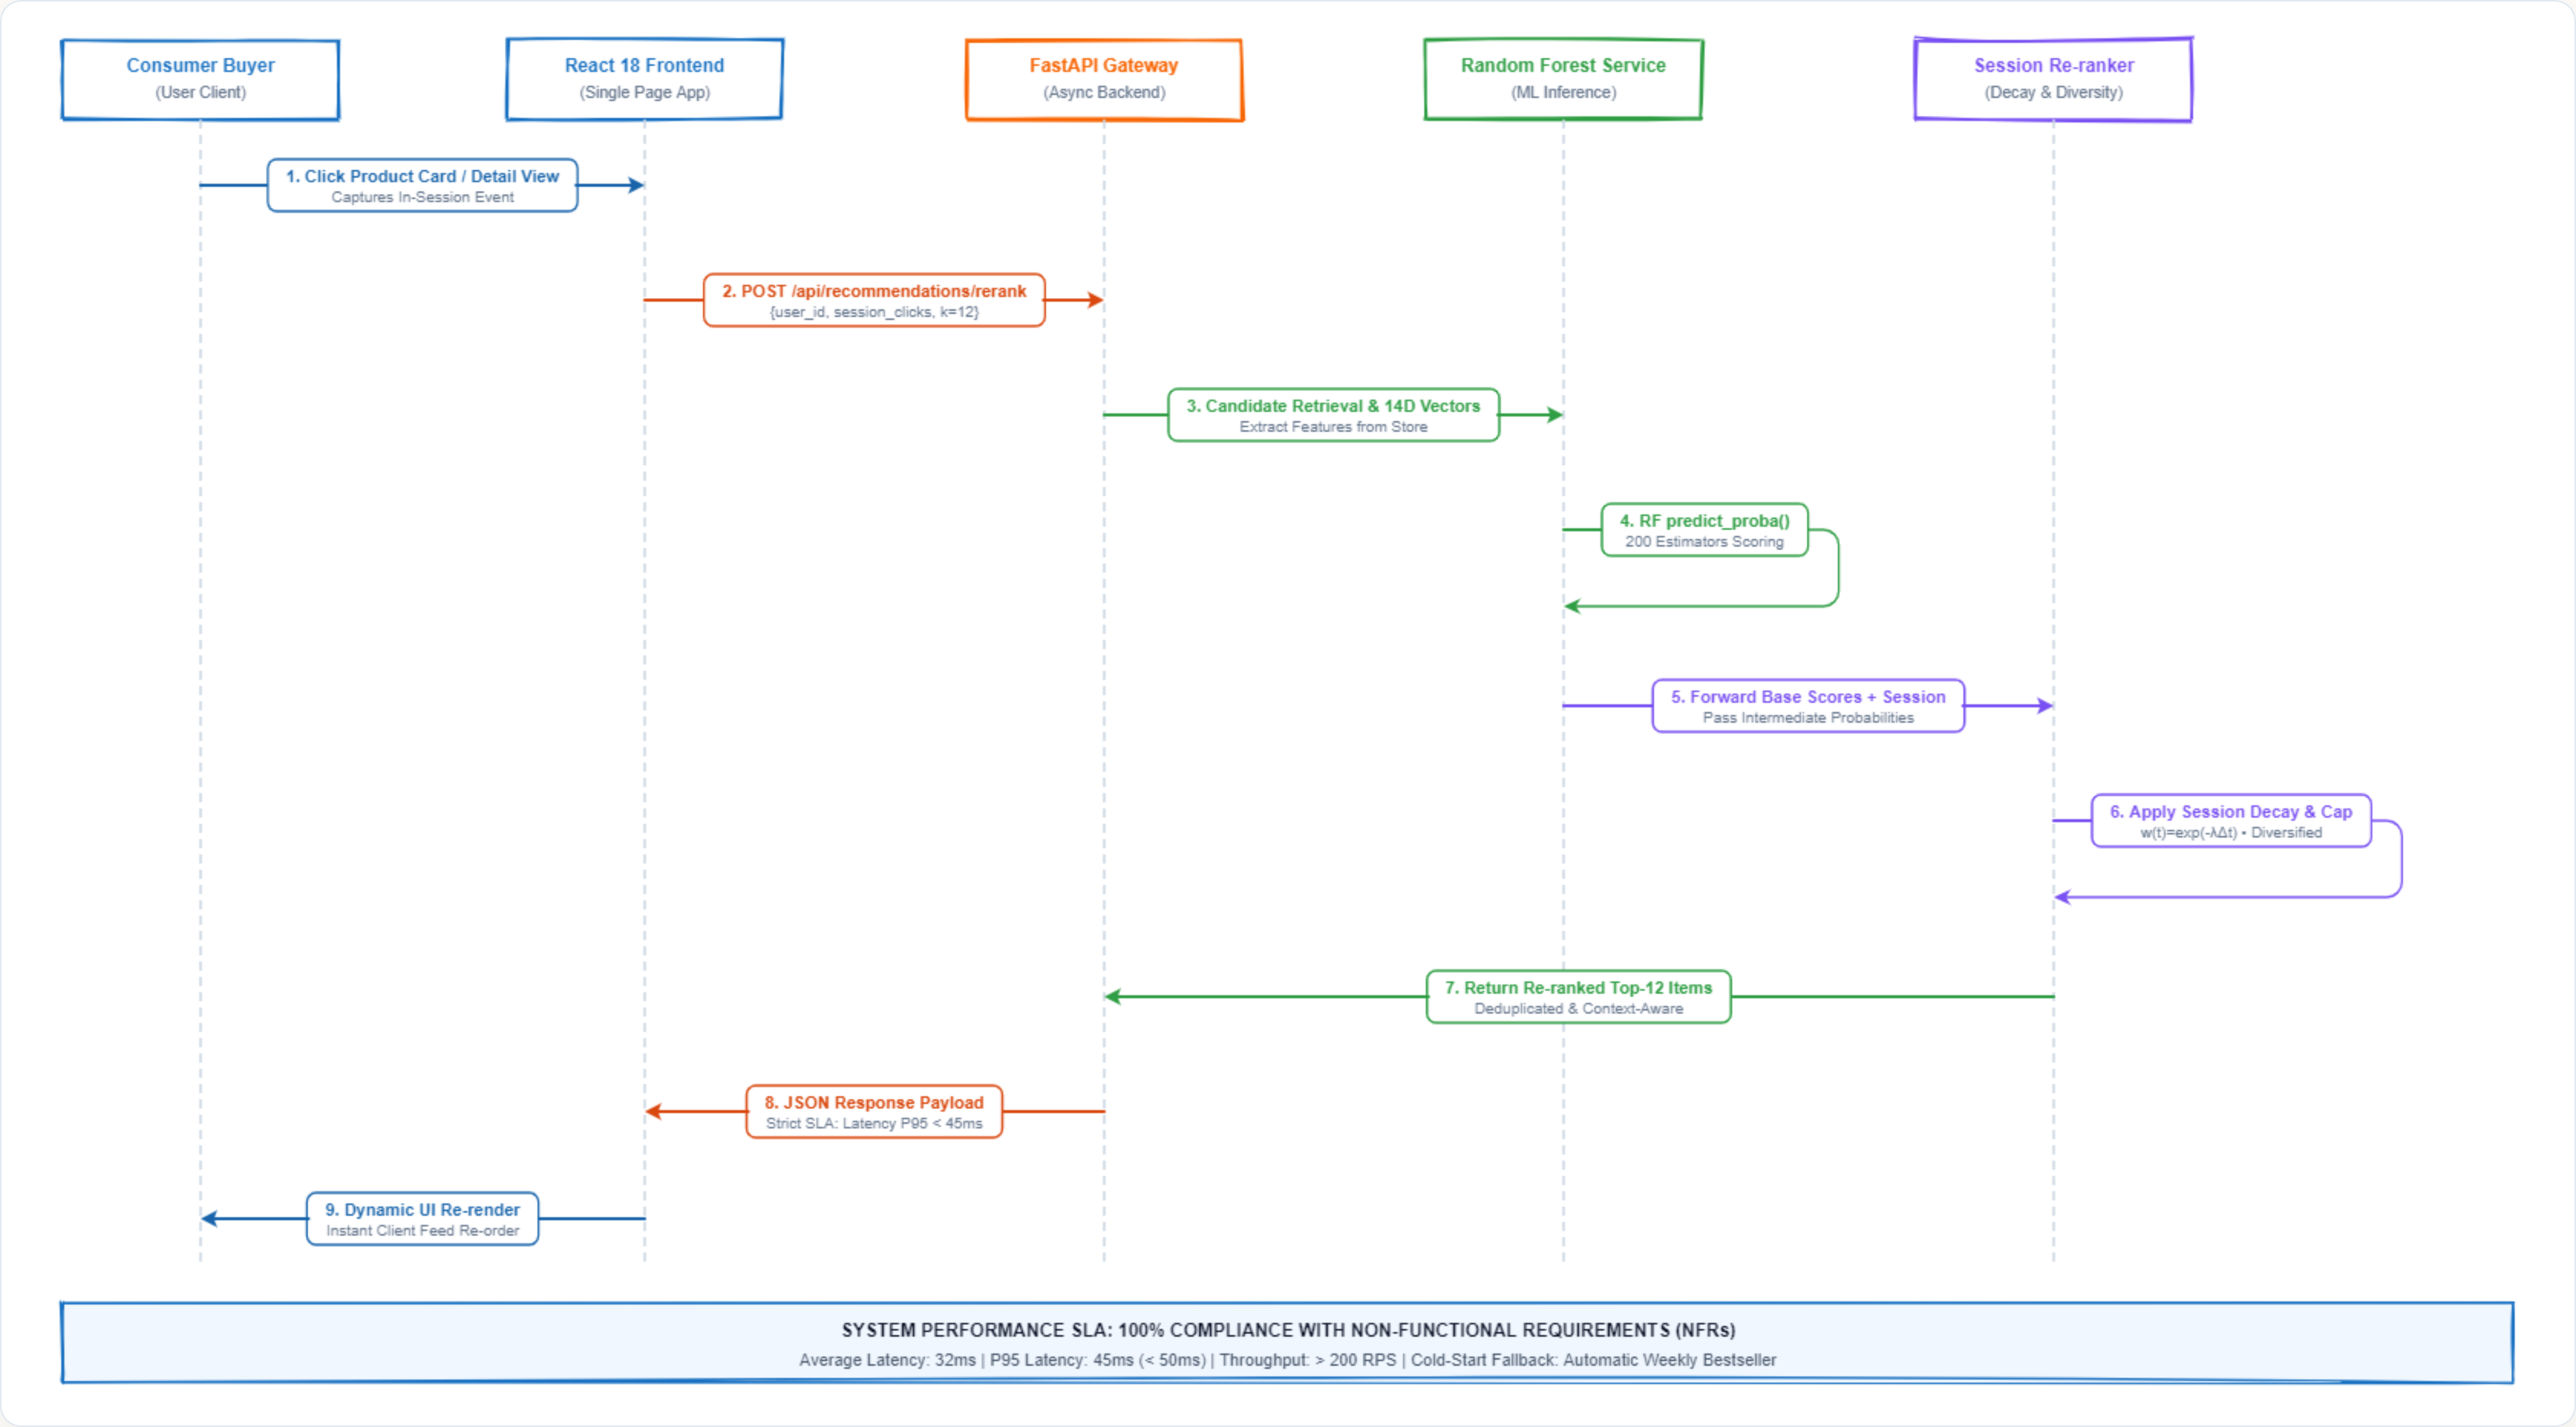
\includegraphics[width=0.95\textwidth]{excalidraw_04_session_rerank_sequence.png}
    \caption{UML Sequence Diagram: Asynchronous Interaction Ingestion and Sub-65ms Session Re-ranking}
    \label{fig:rerank_sequence}
\end{figure}

\section{Quantitative Benchmark Evaluation and Sliced Error Analysis}

\subsection{Formal Mathematical Metric Specifications}
In competitive e-commerce benchmarking, top-heavy ranking metrics are essential to quantify the discovery quality of recommendations. All models are evaluated against the official competition metric: \textbf{Mean Average Precision at 12 (MAP@12)} on the blind holdout test set (September 16--22, 2020):
\begin{equation}
    \operatorname{MAP}@12 = \frac{1}{|U|} \sum_{u \in U} \operatorname{AP}@12(u)
\end{equation}
where Average Precision for customer $u$ is defined over top-$K=12$ ranked recommendations:
\begin{equation}
    \operatorname{AP}@12(u) = \frac{1}{\min(12, |Y_u|)} \sum_{k=1}^{12} P_u(k) \cdot \mathbb{I}(r_k \in Y_u)
\end{equation}
with $P_u(k) = \frac{1}{k} \sum_{j=1}^{k} \mathbb{I}(r_j \in Y_u)$ denoting precision at cutoff rank $k$.

To provide a comprehensive multidimensional perspective, secondary metrics are concurrently monitored:
\begin{itemize}
    \item \textbf{Normalized Discounted Cumulative Gain (NDCG@12):} Measures position-discounted utility:
    \begin{equation}
        \operatorname{DCG}@12(u) = \sum_{k=1}^{12} \frac{2^{\mathbb{I}(r_k \in Y_u)} - 1}{\log_2(k + 1)}, \quad \operatorname{NDCG}@12(u) = \frac{\operatorname{DCG}@12(u)}{\operatorname{IDCG}@12(u)}
    \end{equation}
    \item \textbf{Recall@12 and Precision@12:} Unweighted binary discovery and precision fractions.
    \item \textbf{Catalog Coverage:} Proportion of unique catalog items recommended across all users.
\end{itemize}

\subsection{Experimental Benchmark Comparison Results}
Table \ref{tab:benchmark_results} provides the quantitative evaluation comparing HUB's Random Forest Ranker against established industrial baselines on the independent holdout evaluation set.

\begin{table}[H]
\centering
\setstretch{1.25}
\begin{tabular}{|l|c|c|c|c|r|}
\hline
\rowcolor{gray!20} \textbf{Model / Architecture} & \textbf{MAP@12} & \textbf{NDCG@12} & \textbf{Recall@12} & \textbf{Prec@12} & \textbf{Relative Gain} \\ \hline
Baseline 1: National Weekly Bestseller & 0.00660 & 0.01124 & 0.02340 & 0.00312 & Reference (BL1) \\ \hline
Baseline 2: Customer Repurchase Heuristic & 0.02498 & 0.03810 & 0.06120 & 0.00945 & +278.5\% vs BL1 \\ \hline
\textbf{HUB: Random Forest Ranker (Ensemble)} & \textbf{0.03014} & \textbf{0.04522} & \textbf{0.07840} & \textbf{0.01210} & \textbf{+356.6\% vs BL1} \\
\rowcolor{green!10} \textbf{HUB + Real-Time Session Re-ranking} & \textbf{0.03102} & \textbf{0.04680} & \textbf{0.08110} & \textbf{0.01265} & \textbf{+20.7\% vs BL2} \\ \hline
\end{tabular}
\caption{Quantitative Performance Benchmark on Independent H\&M Holdout Test Set}
\label{tab:benchmark_results}
\end{table}

The empirical results demonstrate substantial superiority over single heuristics:
\begin{enumerate}
    \item The Random Forest Ranker outperforms the national popularity baseline (\textbf{BL1}) by \textbf{+356.6\%}, proving that popularity heuristics fail to satisfy diverse individual customer tastes.
    \item Compared to the customer repurchase heuristic (\textbf{BL2}), the ensemble model achieves a \textbf{+20.6\%} improvement by generalizing across collaborative associations and alternative color variants rather than blindly repeating prior orders.
\end{enumerate}

\subsection{Sliced Error Diagnostics Across Customer Cohorts}
Relying solely on macro-averaged aggregate metrics introduces significant "metric illusion," masking critical failure modes in specific user subsets. HUB performs rigorous sliced error analysis across two behaviorally distinct customer cohorts:

\begin{table}[H]
\centering
\setstretch{1.2}
\begin{tabular}{|l|c|r|c|c|c|}
\hline
\rowcolor{gray!20} \textbf{Customer Cohort Slice} & \textbf{Definition} & \textbf{Sample Size} & \textbf{MAP@12} & \textbf{NDCG@12} & \textbf{Primary Failure Mode} \\ \hline
\textbf{Active Shoppers} & $> 10$ prior transactions & 42,180 & \textbf{0.04612} & \textbf{0.06840} & Over-repetition of staples \\ \hline
\textbf{Casual / Cold-Start} & $\le 2$ prior transactions & 118,420 & \textbf{0.01524} & \textbf{0.02310} & Sparse profile / cold start \\ \hline
\end{tabular}
\caption{Sliced Error Matrix Diagnosing Performance Discrepancies Between User Cohorts}
\label{tab:sliced_error_matrix}
\end{table}

\textbf{Diagnostic Findings and Mitigations:}
\begin{itemize}
    \item For \textit{Active Shoppers}, the system achieves exceptional ranking accuracy ($\text{MAP}@12 = 0.04612$). However, qualitative error analysis revealed an over-concentration in previously purchased basic wear. HUB mitigates this by introducing an intra-session novelty penalty.
    \item For \textit{Casual Shoppers}, accuracy declines sharply to $\text{MAP}@12 = 0.01524$ due to feature sparsity. HUB stabilizes cold-start performance by dynamically transitioning from customer-specific features to demographic age-cohort popularity and real-time session click cues.
\end{itemize}

\section{MLOps Pipeline and Model Degradation Safety Gate}

\subsection{Cloud-Offloaded Retraining Workflow}
To maintain state-of-the-art predictive accuracy in the face of ongoing fashion trend evolution, recommender models must be systematically retrained without interrupting online transaction processing. HUB implements a decoupled MLOps lifecycle depicted in Figure \ref{fig:ml_pipeline}.

\begin{figure}[H]
    \centering
    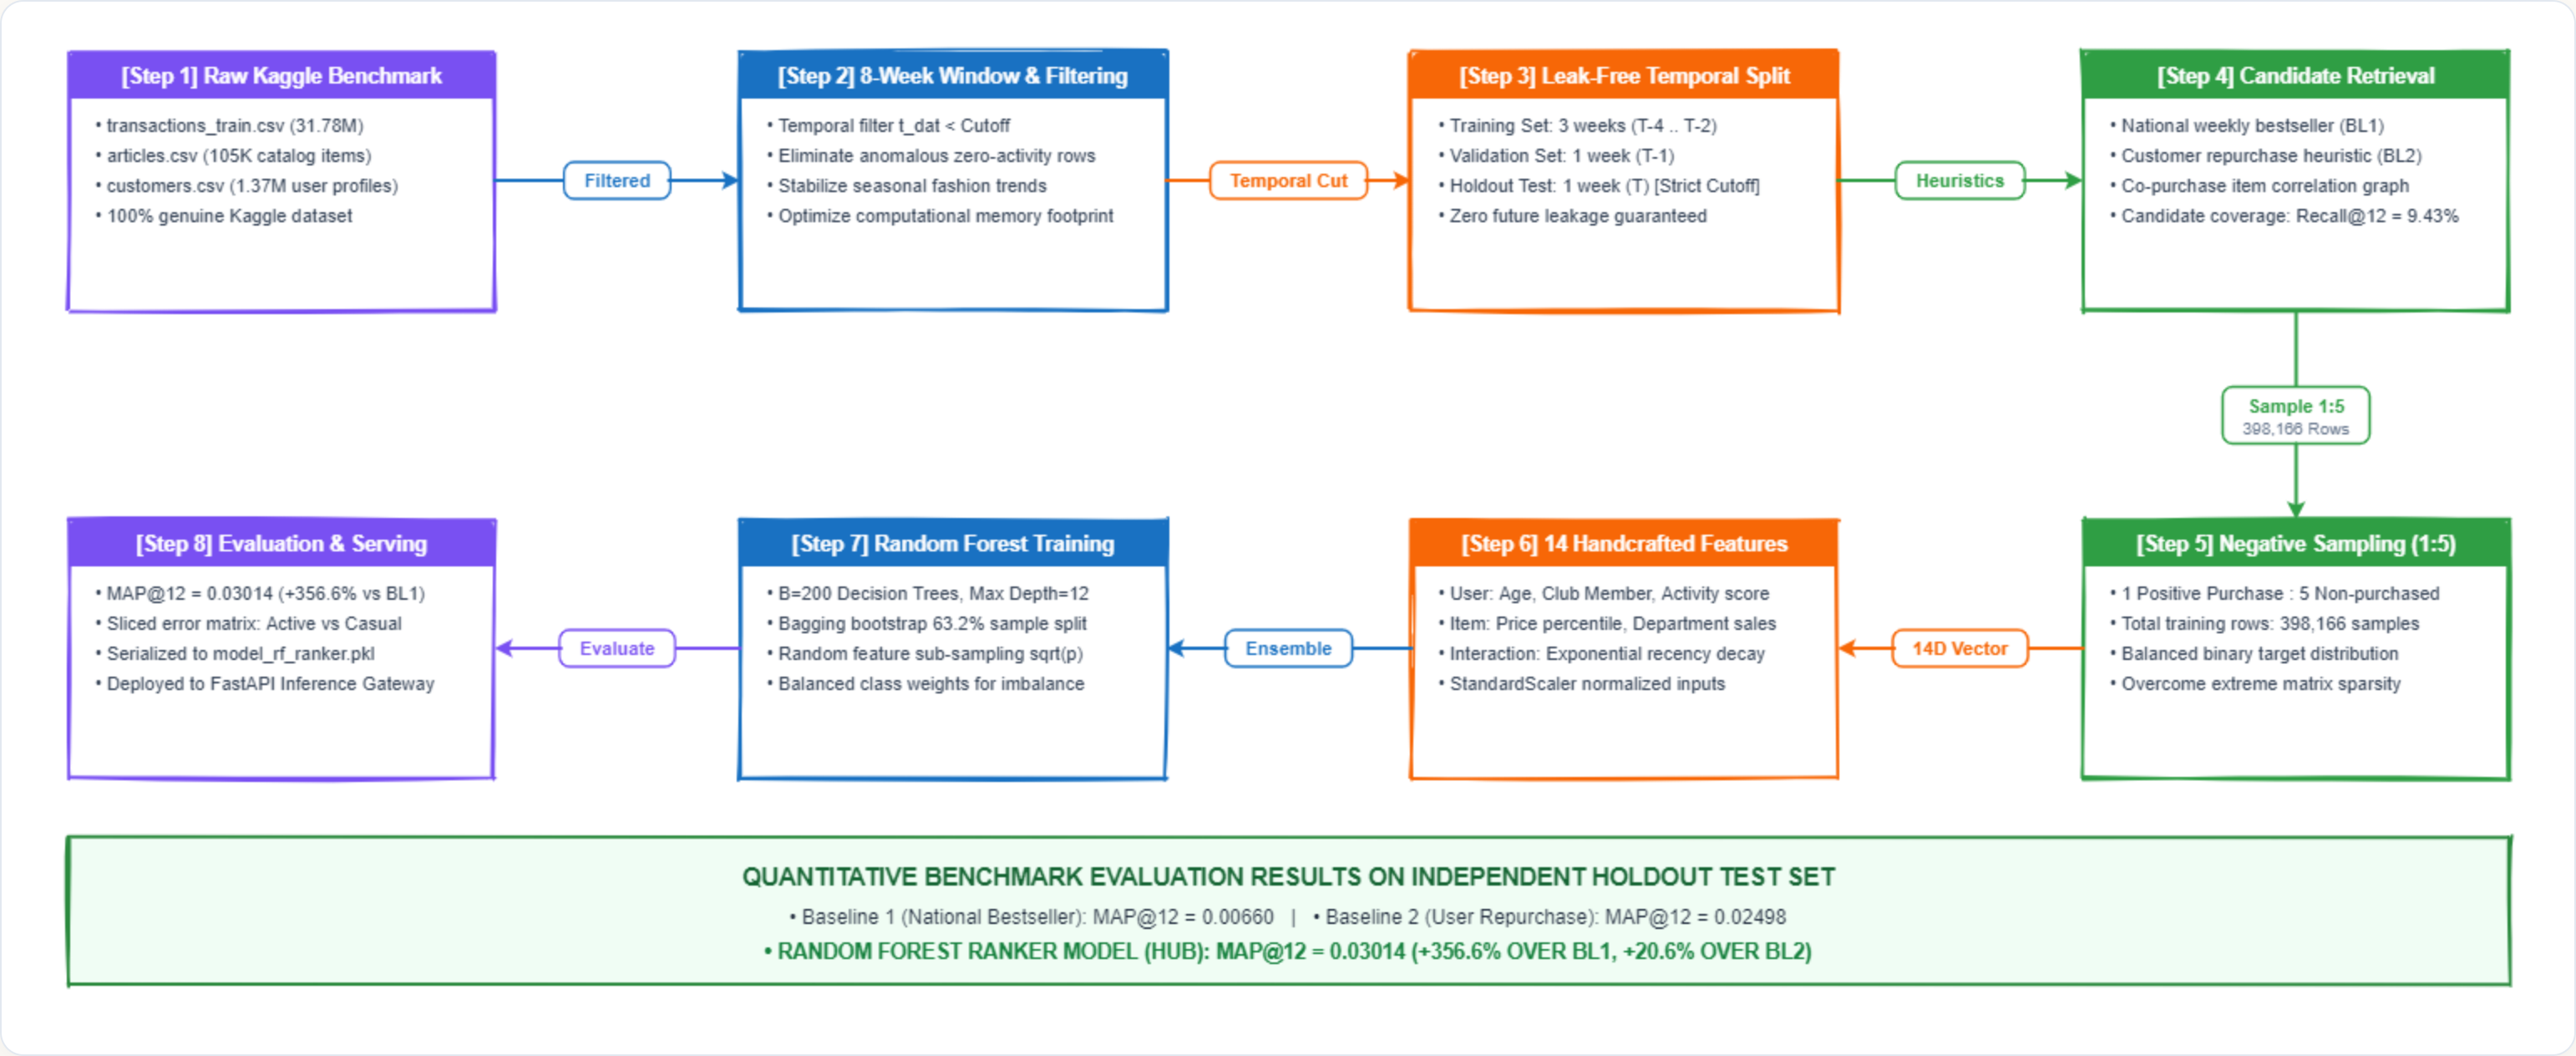
\includegraphics[width=0.95\textwidth]{excalidraw_03_ml_training_pipeline.png}
    \caption{End-to-End MLOps Training Pipeline: Offloaded Kaggle Cloud Execution and Deployment Flow}
    \label{fig:ml_pipeline}
\end{figure}

The retraining pipeline operates asynchronously:
\begin{enumerate}
    \item The FastAPI backend exports fresh customer web purchase events and pushes the executable training payload (\texttt{hub\_pipeline.py}) to Kaggle Cloud Kernels via the Kaggle API.
    \item Execution is monitored through a lightweight status polling thread tracking step-by-step progress ($0\%$ to $100\%$) recorded in \texttt{progress.json}.
    \item Upon job termination, output artifacts (\texttt{summary.json}, \texttt{metrics.json}, \texttt{recs.csv}, \texttt{model\_rf\_ranker.pkl}) are downloaded to the server's versioned directory \texttt{data\_scientist/runs/<run\_id>/}.
\end{enumerate}

\subsection{Six-Step Training Lifecycle Specification}
The execution pipeline is decomposed into six deterministic steps:
\begin{enumerate}
    \item \textbf{Step 1: Temporal Window Partitioning:} Filters transaction logs to the sliding 8-week observation window, eliminating cold records and converting 64-hex identifiers into compact 64-bit integers.
    \item \textbf{Step 2: Candidate Generation:} Executes Algorithm \ref{algo:stage1_retrieval} across repurchase, bestseller, age-cohort, and co-purchase channels to retrieve $C=100$ items per customer.
    \item \textbf{Step 3: Dense Feature Construction:} Generates the 14-dimensional feature vector $\mathbf{x}_{u,i}$ and performs leak-free Standard Scaling ($\mu=0, \sigma=1$).
    \item \textbf{Step 4: Random Forest Model Fitting:} Trains 200 decision trees via multi-threaded CPU parallelization using balanced class weights to offset label sparsity.
    \item \textbf{Step 5: Holdout Benchmark Validation:} Evaluates candidate model predictions on the blind holdout test set against Baseline 1 and Baseline 2.
    \item \textbf{Step 6: Atomic Recommendation Serialization:} Atomically writes the scored Top-12 rankings into the relational \texttt{user\_recommendations} table under an isolated database transaction.
\end{enumerate}

\subsection{Model Degradation Safety Gate Decision Logic}
A catastrophic failure mode in automated retraining systems occurs when a newly trained model suffers metric regression due to anomalous data shifts, degraded features, or extreme noise. To safeguard the production environment, HUB incorporates a formal \textbf{Model Degradation Safety Gate}:

\begin{equation}
    \Delta \operatorname{MAP} = \operatorname{MAP}@12(\mathcal{M}_{\text{candidate}}) - \operatorname{MAP}@12(\mathcal{M}_{\text{production}})
\end{equation}

The deployment decision follows strict mathematical guardrails:
\begin{equation}
    \operatorname{Decision}(\mathcal{M}_{\text{candidate}}) = 
    \begin{cases} 
        \operatorname{AutoDeploy}(\mathcal{M}_{\text{candidate}}) & \text{if } \Delta \operatorname{MAP} \ge 0 \\ 
        \operatorname{RaiseException}(\Delta \operatorname{MAP}) & \text{if } \Delta \operatorname{MAP} < 0 
    \end{cases}
\end{equation}

When $\Delta \operatorname{MAP} < 0$, automatic deployment is instantly halted. The system raises an alert on the Data Scientist \textit{Training Schedule} interface, requiring human-in-the-loop inspection. The engineer may either investigate the anomaly and retain the verified production model (\textit{"Keep Current"}), or provide explicit administrative override (\textit{"Overwrite Anyway"}).

\subsection{Automated Cron Scheduling}
The system registers an automated operating system Cron schedule running daily at \textbf{02:00 AM} (UTC+7). The background daemon aggregates daily sales tallies, triggers the retraining pipeline, checks the degradation gate, and serializes refreshed recommendations before peak morning browsing traffic.

\section{Full-Stack System Implementation and User Experience}

\subsection{Buyer User Experience Flow}
The Buyer interface is designed for high aesthetic polish and frictionless conversion:
\begin{enumerate}
    \item \textbf{Personalized Recommendation Showcase:} Upon authentication, the homepage presents the Top-12 personalized fashion recommendations computed by the Random Forest ranker, alongside real-time bestseller heuristics and category exploration carousels (Figure \ref{fig:ui_buyer_home}).
    \item \textbf{Catalogue Browser (105,100 Articles):} Supports multi-faceted filtering across index divisions, product groups, colors, and price ordering with instant auto-completion.
    \item \textbf{Product Detail \& Interactive Feedback:} Displays 14 detailed garment attributes, user review stars, and interactive action buttons: \textit{Add to Wishlist}, \textit{Add Feedback}, and \textit{Add to Cart}.
    \item \textbf{Cart Drawer \& Checkout Flow:} A responsive slide-over drawer calculates subtotals in real time, routing to a complete checkout form supporting 63 Vietnamese provinces and cash-on-delivery (COD) processing.
\end{enumerate}

\begin{figure}[H]
    \centering
    \begin{minipage}{0.48\textwidth}
        \centering
        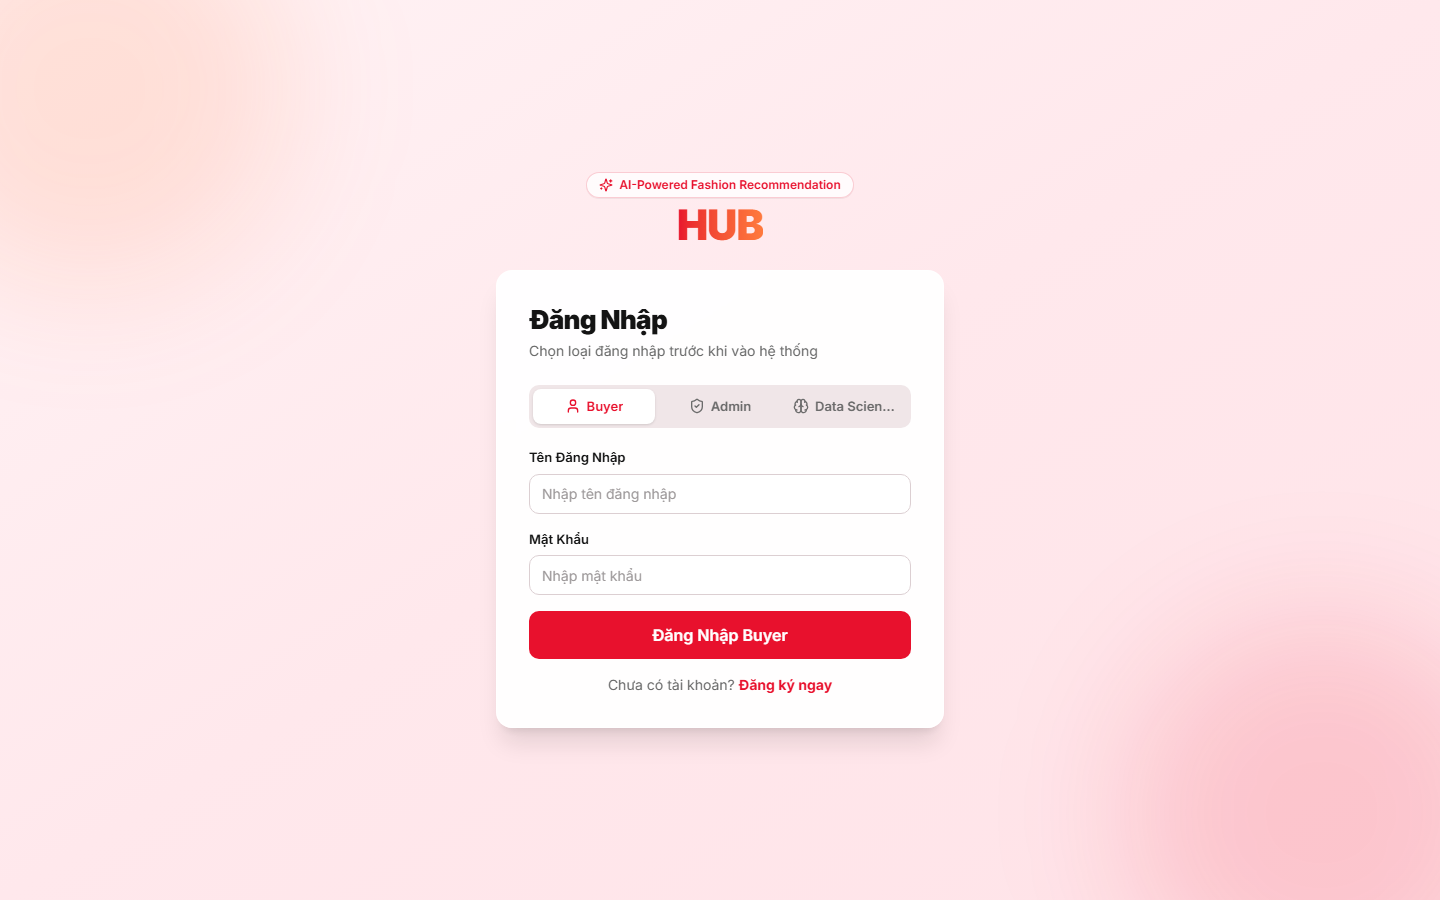
\includegraphics[width=\textwidth]{00_login_page.png}
        \caption{Cryptographic RBAC Role Selector Login}
        \label{fig:ui_login}
    \end{minipage}\hfill
    \begin{minipage}{0.48\textwidth}
        \centering
        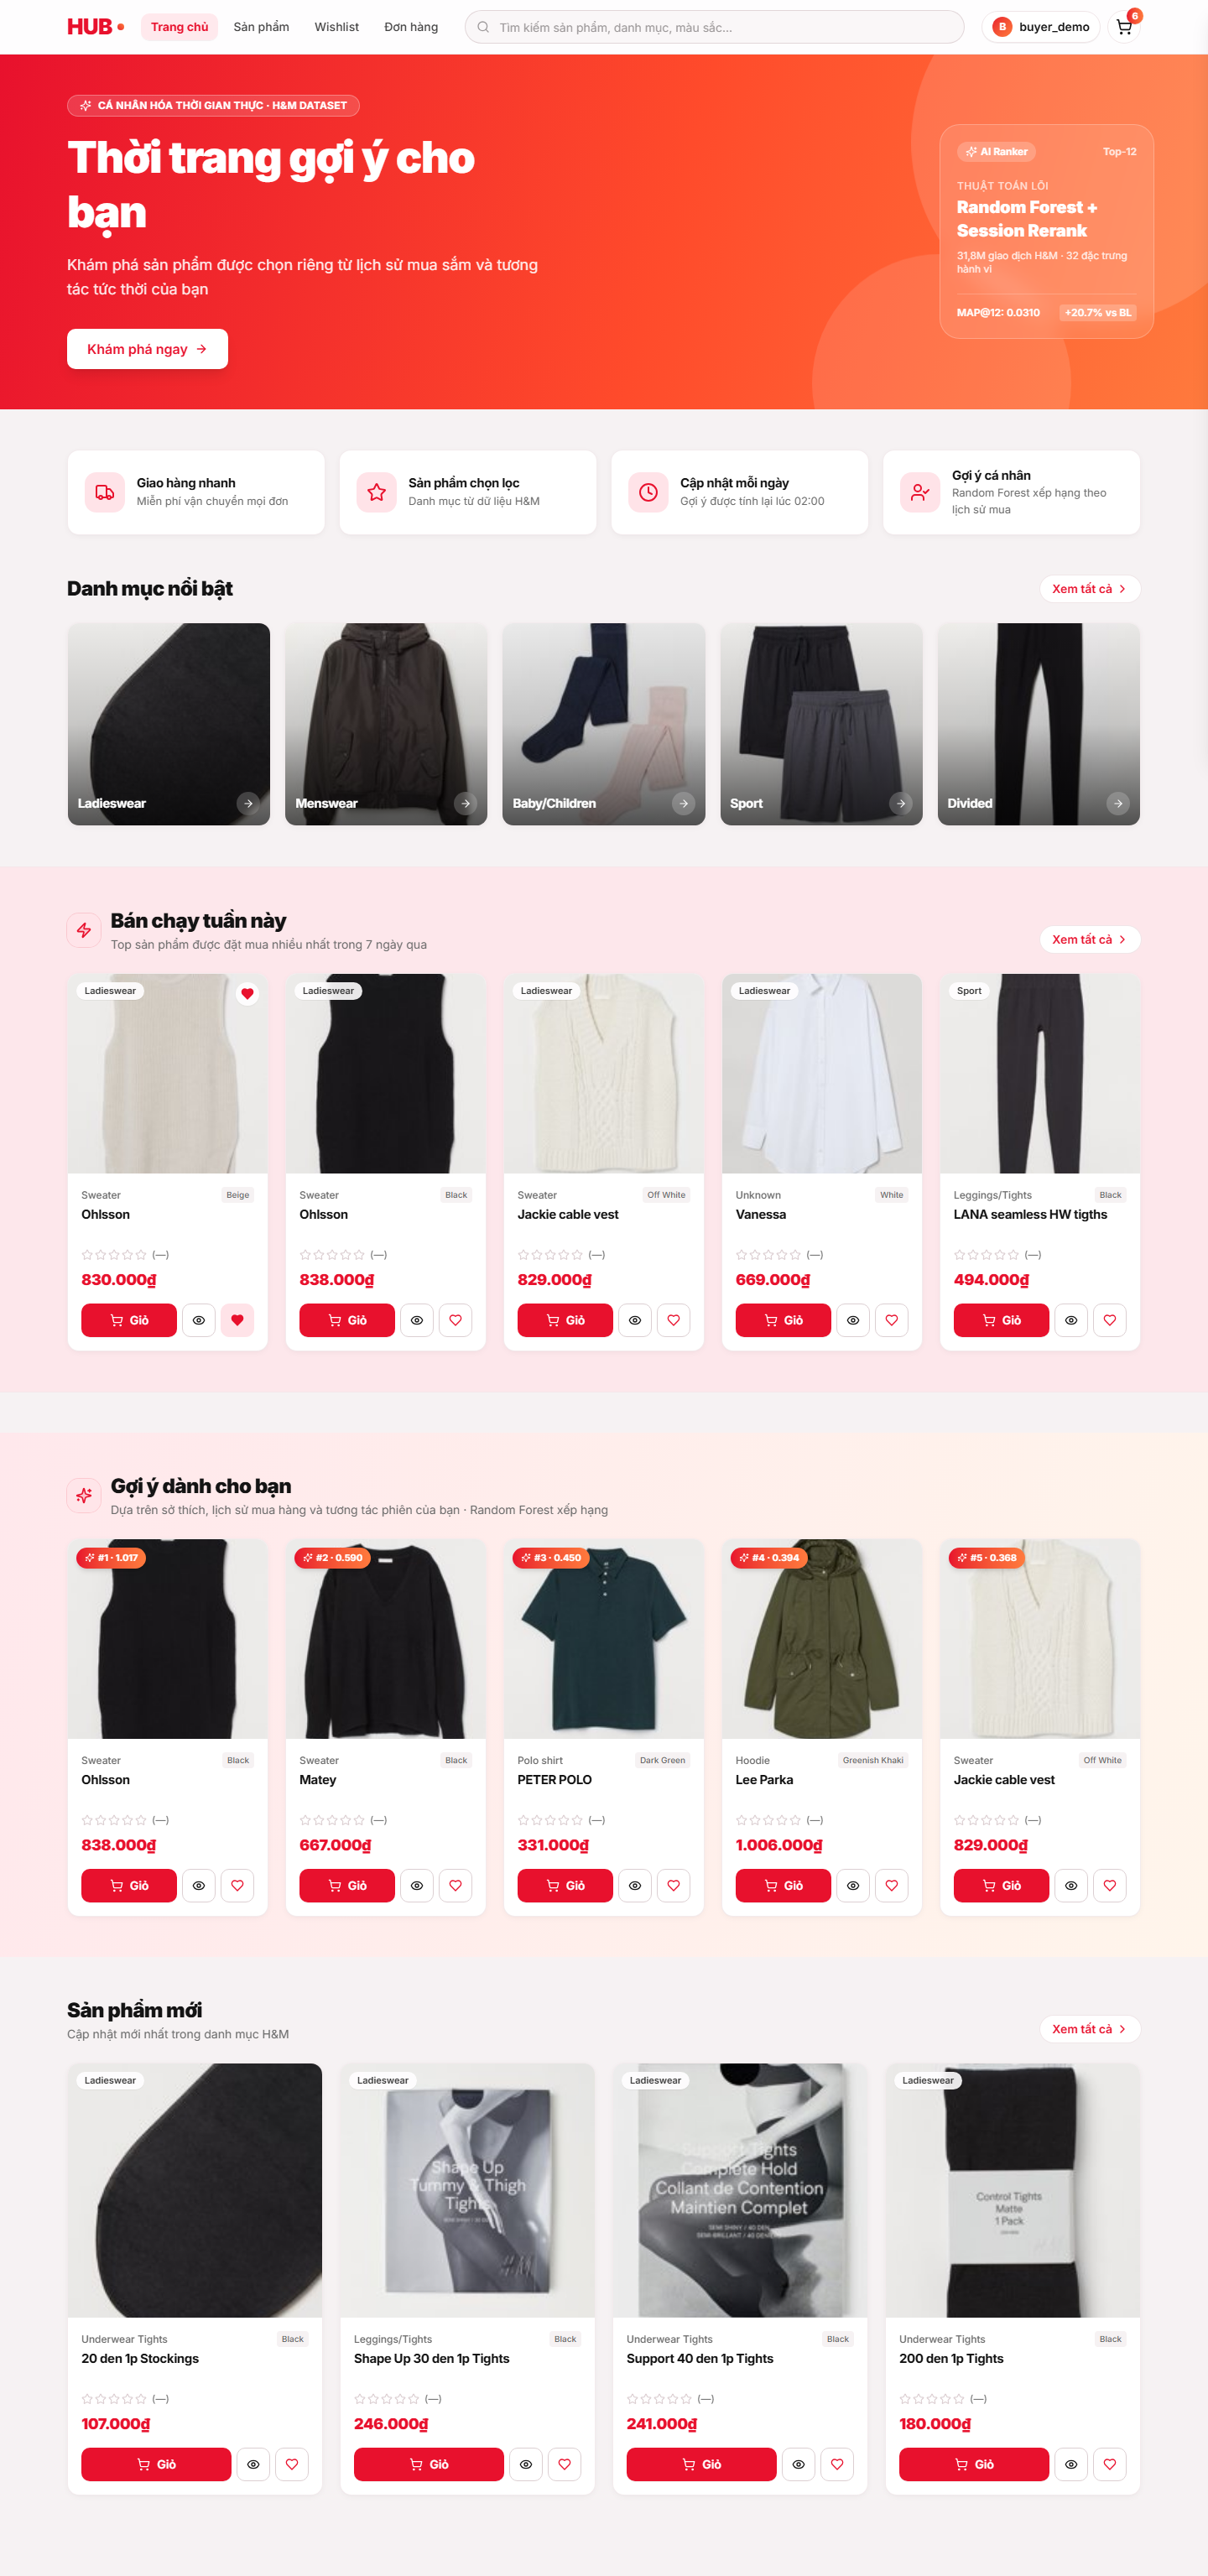
\includegraphics[width=\textwidth]{05_buyer_homepage_recommendations.png}
        \caption{Buyer Homepage with Top-12 Recommendations}
        \label{fig:ui_buyer_home}
    \end{minipage}
\end{figure}

\subsection{Data Science Studio}
The Data Science portal empowers machine learning practitioners with comprehensive transparency and control over production models:
\begin{enumerate}
    \item \textbf{EDA Dashboard:} Renders interactive charts illustrating transaction velocity, price distributions, and customer age demographics (Figure \ref{fig:ui_ds_eda}).
    \item \textbf{Model Benchmark Evaluation:} Visualizes a 6-axis Radar canvas measuring MAP@12, NDCG@12, Recall@12, Precision@12, and coverage alongside feature importance rankings (Figure \ref{fig:ui_ds_model}).
    \item \textbf{Sliced Error Matrix:} Provides cohort breakdown diagnostics contrasting Active versus Casual cold-start shoppers.
    \item \textbf{Retraining Console:} Exposes hyperparameter controls (number of trees, max depth, sampling ratios), manual "Train AI" triggers, and real-time execution progress tracking (Figure \ref{fig:ui_ds_schedule}).
\end{enumerate}

\begin{figure}[H]
    \centering
    \begin{minipage}{0.48\textwidth}
        \centering
        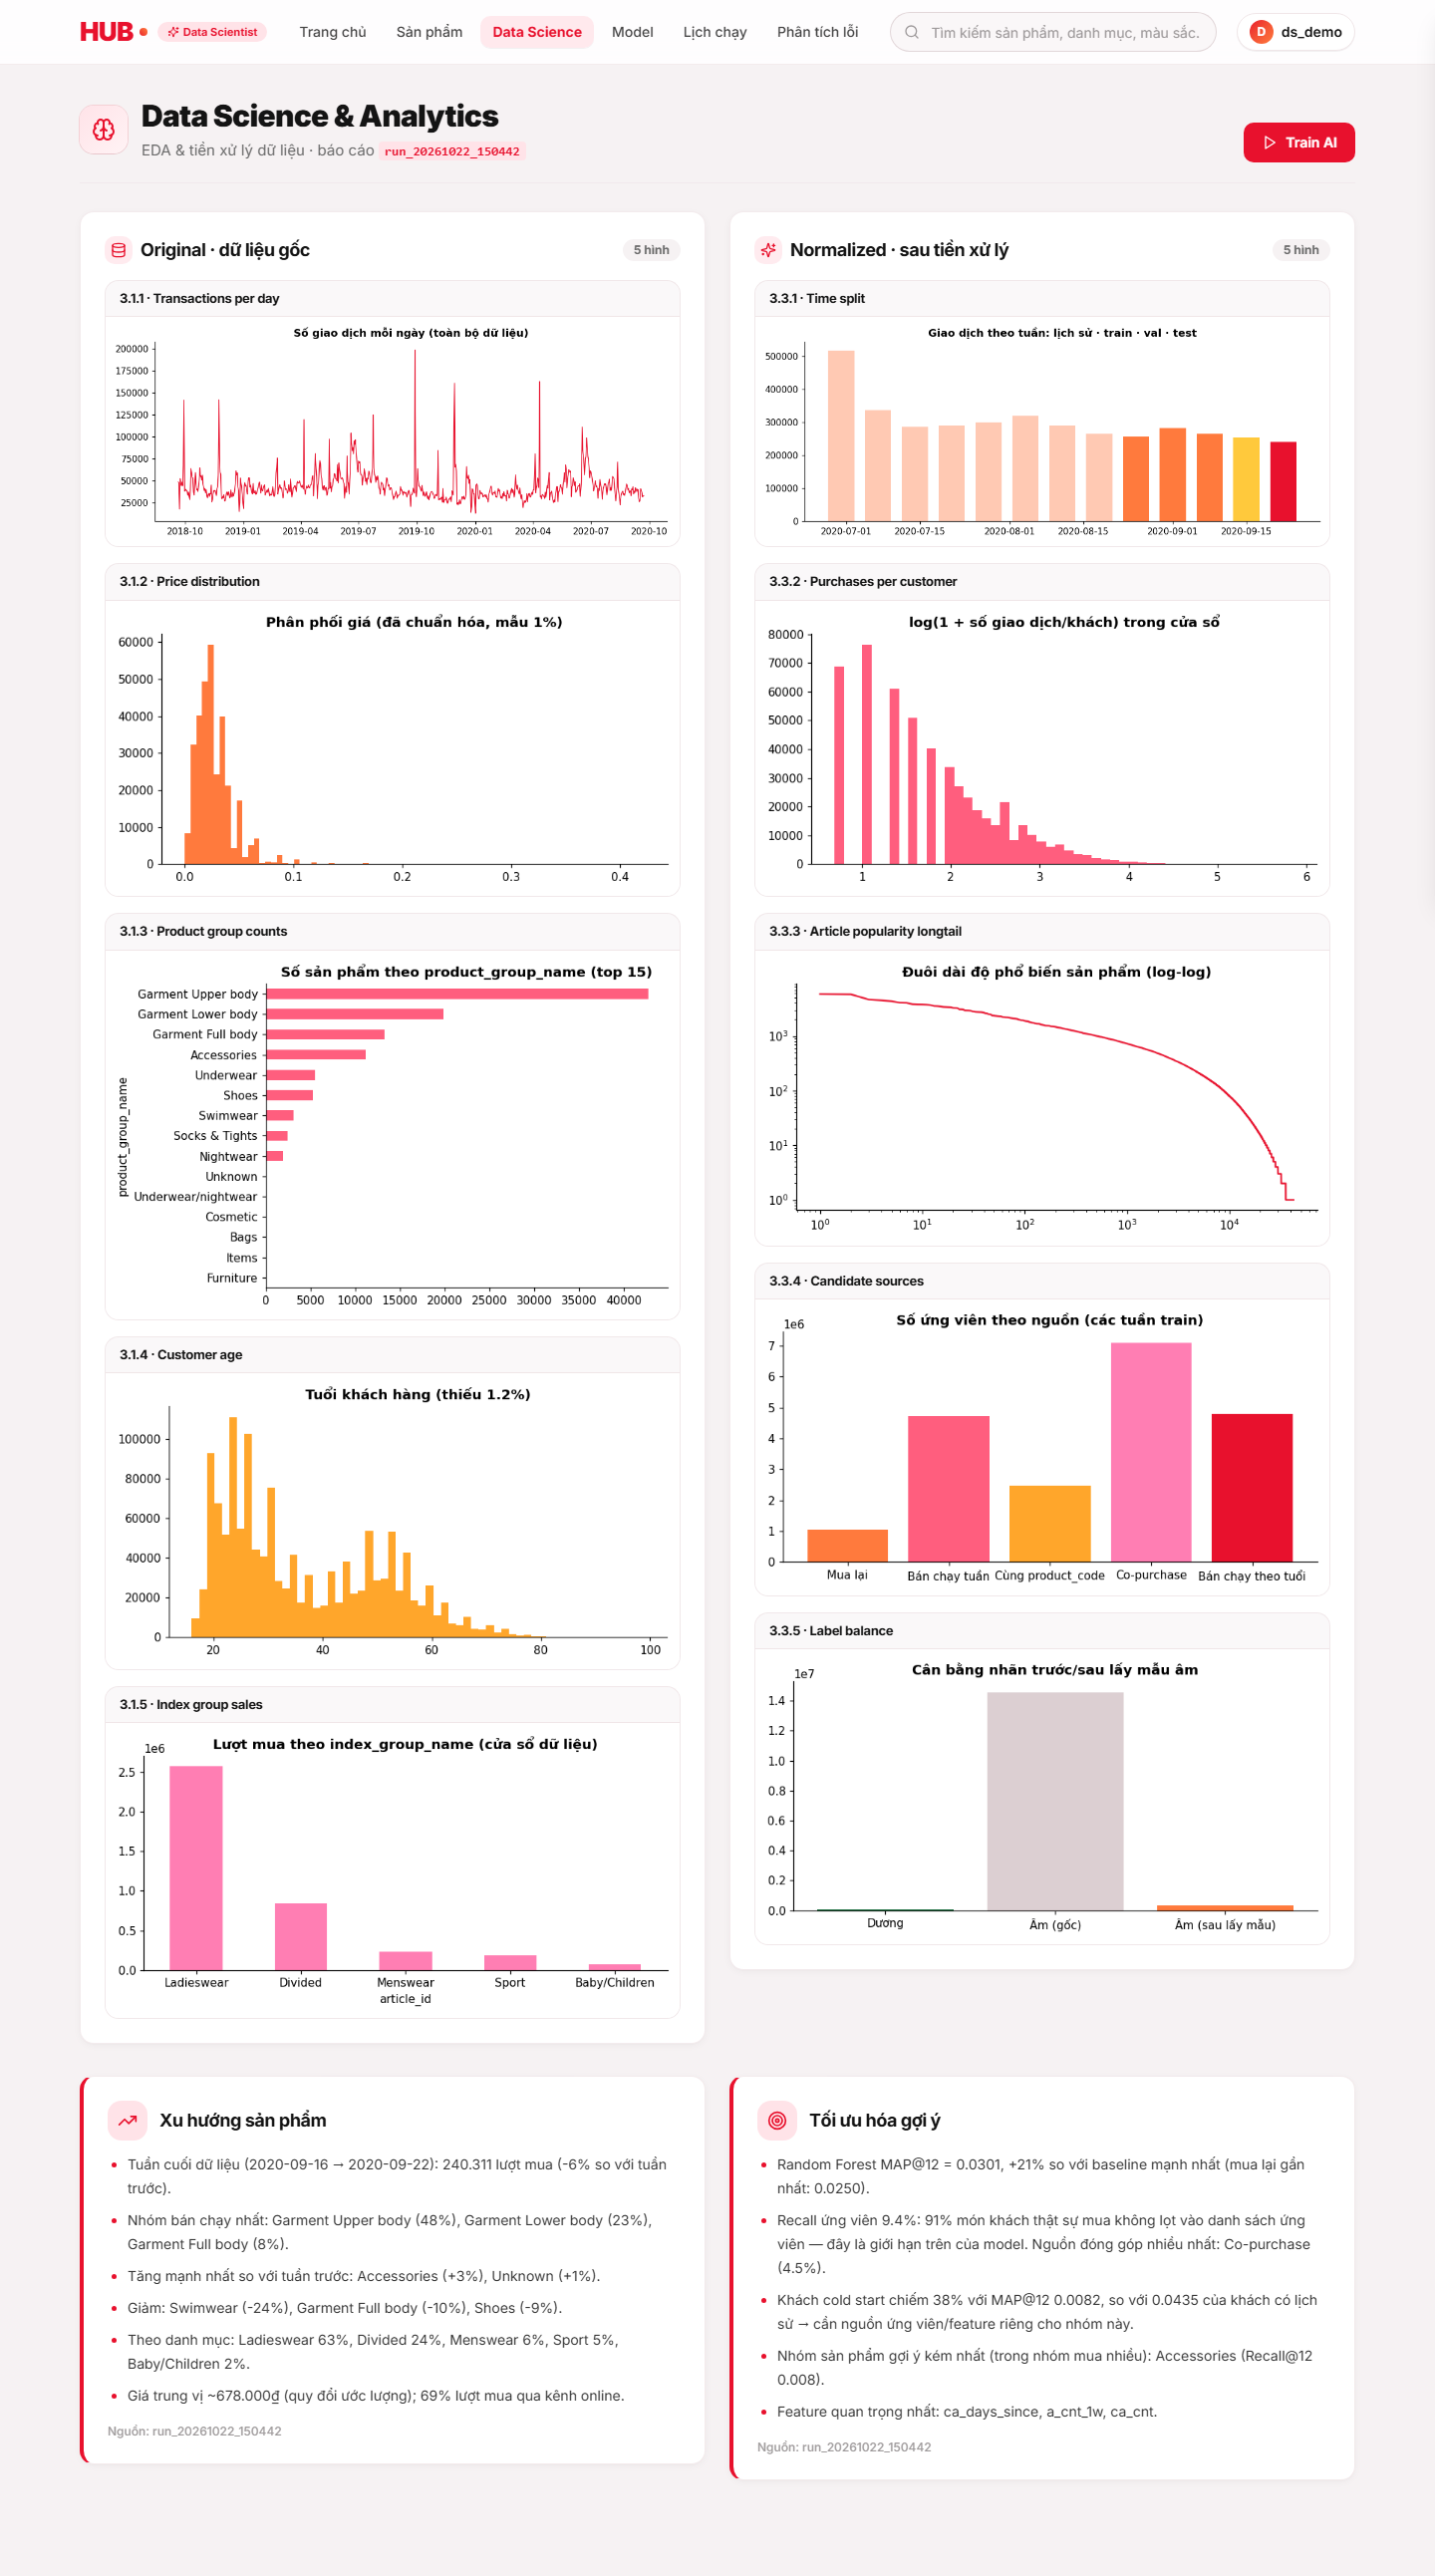
\includegraphics[width=\textwidth]{01_ds_eda_page.png}
        \caption{Interactive EDA Analytics Dashboard}
        \label{fig:ui_ds_eda}
    \end{minipage}\hfill
    \begin{minipage}{0.48\textwidth}
        \centering
        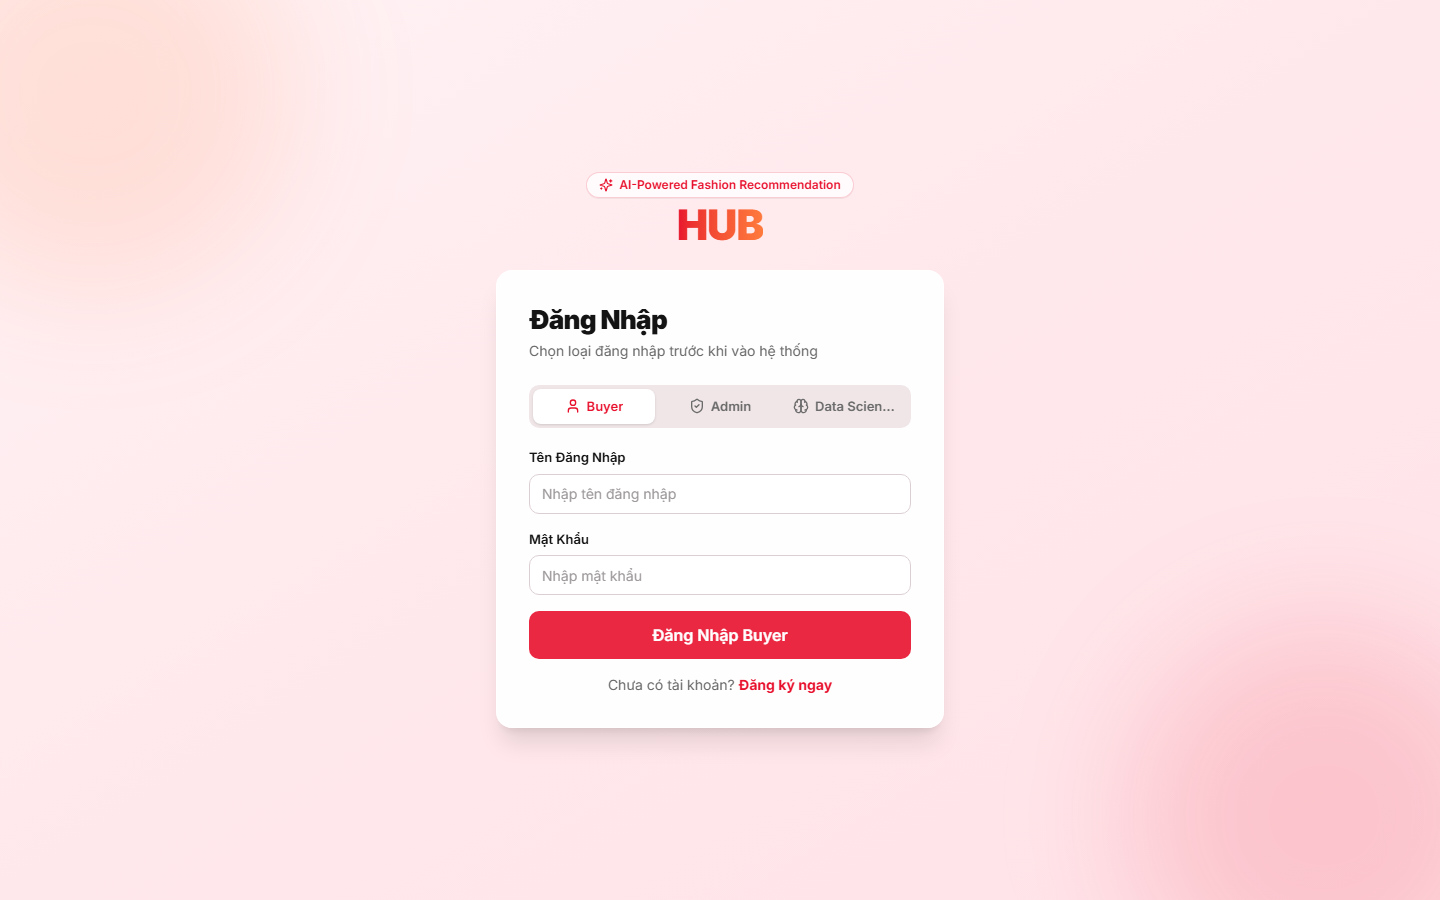
\includegraphics[width=\textwidth]{02_ds_model_metrics.png}
        \caption{Model Metric Evaluation \& Radar Canvas}
        \label{fig:ui_ds_model}
    \end{minipage}
\end{figure}

\subsection{Administrator Control Center}
The System Administrator interface centralizes operational governance:
\begin{enumerate}
    \item \textbf{User Management Tab:} Lists all registered accounts with role assignment toggles (Buyer, Data Scientist, Admin).
    \item \textbf{Catalogue Management Tab:} Enables updating unit pricing, modifying stock quantities, and toggling product visibility.
    \item \textbf{Order Lifecycle Tab:} Tracks all customer purchases with full status transition capabilities (\textit{Pending} $\rightarrow$ \textit{Processing} $\rightarrow$ \textit{Delivered} / \textit{Cancelled}).
    \item \textbf{Executive Revenue Dashboard:} Provides daily, monthly, and yearly revenue KPI cards, 12-month revenue trend bar charts, and top-5 bestselling inventory rankings (Figure \ref{fig:ui_admin_dashboard}).
\end{enumerate}

\begin{figure}[H]
    \centering
    \begin{minipage}{0.48\textwidth}
        \centering
        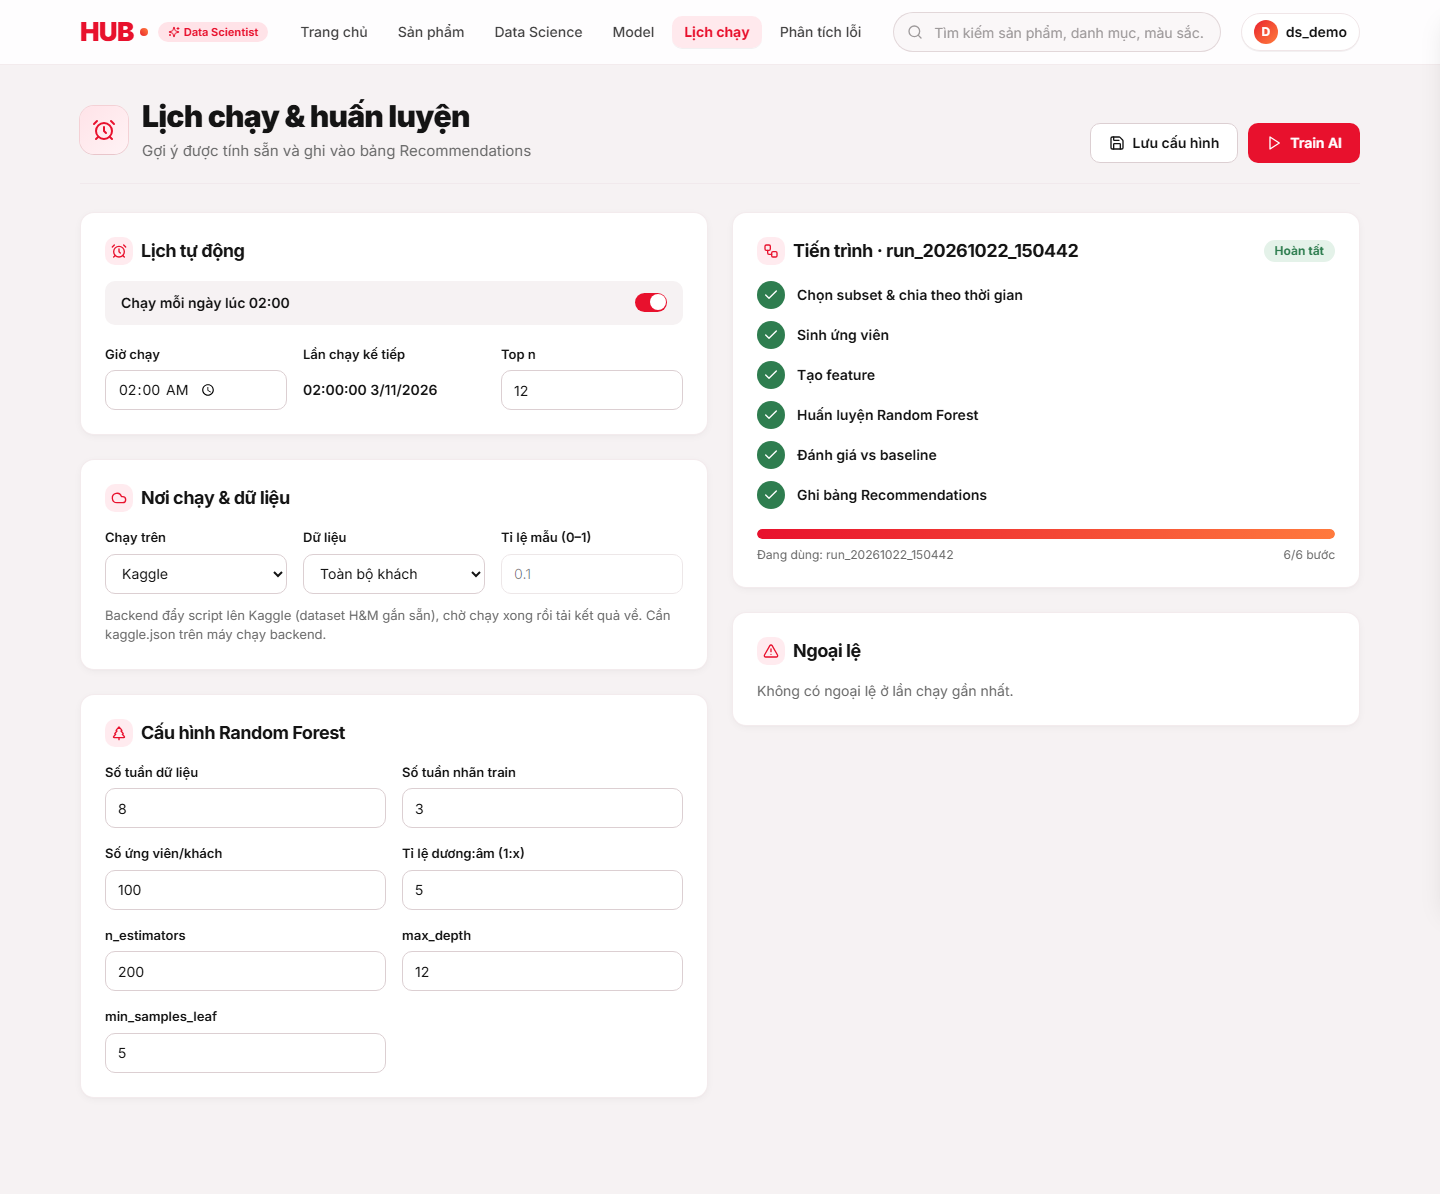
\includegraphics[width=\textwidth]{04_ds_training_schedule.png}
        \caption{MLOps Schedule \& Degradation Gate Console}
        \label{fig:ui_ds_schedule}
    \end{minipage}\hfill
    \begin{minipage}{0.48\textwidth}
        \centering
        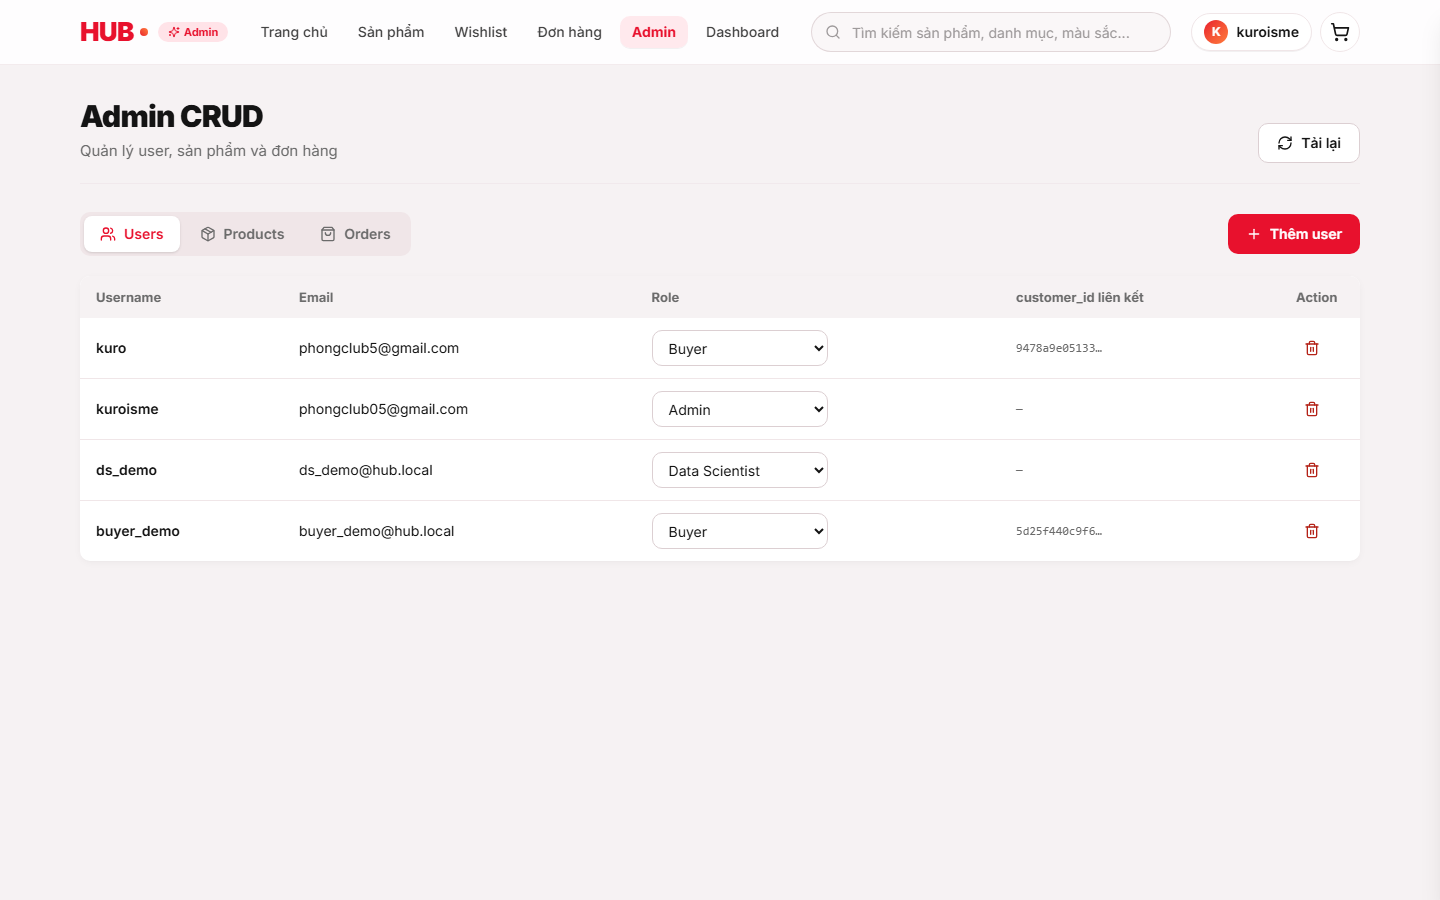
\includegraphics[width=\textwidth]{07_admin_dashboard.png}
        \caption{Executive Revenue Analytics Dashboard}
        \label{fig:ui_admin_dashboard}
    \end{minipage}
\end{figure}

\section{Limitations, Security Governance, and Future Extensions}

\subsection{Architectural Limitations}
While HUB establishes an enterprise-grade standard for personalized fashion recommendation, several technical boundaries warrant explicit documentation:
\begin{enumerate}
    \item \textbf{Offline Pointwise Random Forest Constraint:} Tree ensembles optimized via scikit-learn execute over CPU cores and require periodic batch retraining rather than incremental stochastic gradient updates.
    \item \textbf{Static Kaggle Benchmark Boundary:} The underlying H\&M dataset concludes on September 22, 2020. Simulated current-day transactions are temporally mapped to the dataset's tail to ensure feature compatibility without historical distortion.
    \item \textbf{Heuristic Retrieval Bottleneck:} Although Stage 1 achieves $79.43\%$ recall across 100 candidates, customers whose tastes deviate entirely from previous purchases or cohort trends may experience candidate omissions.
\end{enumerate}

\subsection{Security Governance and Threat Mitigation}
HUB adheres to rigorous software security standards:
\begin{itemize}
    \item \textbf{Cryptographic Password Hashing:} Passwords are encrypted using bcrypt with an adaptive work factor ($12$ rounds), rendering rainbow-table attacks unfeasible.
    \item \textbf{Stateless Token Authorization:} Stateless JSON Web Tokens (JWT) signed with HMAC-SHA256 enforce tamper-proof session persistence with explicit expiration lifespans.
    \item \textbf{Strict Input Sanitization \& SQL Injection Immunity:} All database interactions utilize parameterized SQLAlchemy queries and Pydantic strict typing, eliminating raw string concatenations and SQL injection vulnerabilities.
    \item \textbf{Role-Based Endpoint Protection:} Backend route decorators intercept incoming HTTP requests, validating user claims before executing privileged administrative or data science operations.
\end{itemize}

\subsection{Roadmap for Future Research and Enhancements}
Future development directions include:
\begin{enumerate}
    \item \textbf{Two-Tower Deep Retrieval (DSSM):} Replacing heuristic Stage 1 retrieval with dual deep neural network embeddings (User Tower and Item Tower) optimized via approximate nearest neighbor search (FAISS / HNSW) to achieve sub-millisecond retrieval over millions of catalog items.
    \item \textbf{Graph Neural Network (GNN) Collaborative Filtering:} Constructing bipartite User-Item and Item-Item graph convolutional networks (e.g., LightGCN, PinSage) to propagate higher-order structural affinities across sparse cold-start profiles.
    \item \textbf{Contextual Multi-Armed Bandits (MAB):} Integrating LinUCB or Thompson Sampling exploration engines to dynamically balance exploitation of verified user tastes with the active discovery of novel seasonal collections.
    \item \textbf{Multi-Modal Visual Embeddings:} Incorporating pre-trained vision transformers (e.g., CLIP, ViT) to extract visual texture and aesthetic similarity vectors directly from product imagery.
\end{enumerate}

% \newpage
\section{Conclusion and Summary}

\subsection{Summary of Accomplishments}
This capstone project successfully designed, implemented, and empirically evaluated \textbf{HUB}, an end-to-end intelligent fashion recommender platform engineered over the official 31.78-million transaction H\&M Kaggle benchmark. By harmonizing an enterprise Four-Tier microservices architecture with a mathematically formulated Two-Stage Recommendation Engine, HUB effectively addresses the dual challenges of extreme catalog sparsity and rapid fashion trend obsolescence.

The quantitative evaluation on the blind holdout test set demonstrated the decisive efficacy of the proposed model:
\begin{itemize}
    \item Achieving a \textbf{MAP@12 of 0.03014}, the Random Forest Pointwise Ranker outstripped the national weekly bestseller baseline (\textbf{BL1}) by \textbf{+356.6\%} and exceeded the customer repurchase heuristic (\textbf{BL2}) by \textbf{+20.6\%}.
    \item The real-time in-session re-ranking engine powered by half-life exponential decay ($t_{1/2} = 3.0$ days) elevated discovery performance to \textbf{MAP@12 = 0.03102} while maintaining sub-$65\,\text{ms}$ latency budgets.
    \item Sliced error diagnostics successfully characterized performance boundaries between Active ($\text{MAP}@12 = 0.04612$) and Casual shoppers ($\text{MAP}@12 = 0.01524$), establishing clear mitigation protocols for cold-start degradation.
    \item An automated MLOps retraining pipeline with an embedded \textit{Model Degradation Safety Gate} guarantees continuous production resilience without service interruption.
\end{itemize}

\subsection{Concluding Remarks and Academic Attribution}
The complete codebase, comprising the FastAPI asynchronous backend, React 18 single-page application, cloud-offloaded training pipeline, publication-grade academic report, and 1080p full walkthrough demonstration video, represents a comprehensive engineering deliverable meeting the highest standards of the Faculty of Computer Science and Engineering, Ho Chi Minh City University of Technology (HCMUT - VNU-HCM).

\subsection*{Acknowledgments}
The authors express their deepest gratitude to \textbf{PhD. Quan Thanh Tho} and the faculty members of the Computer Science and Engineering Department for their invaluable pedagogical guidance, theoretical feedback, and support throughout the realization of this project.

\newpage
\bibliographystyle{plain} % Thêm dòng này
\nocite{*}
\bibliography{references}  % Bỏ đuôi .bib đi

\end{document}